%-----------------------------------------------------------------------
% Beginning of mcom-l-template.tex
%-----------------------------------------------------------------------
%
%     This is a topmatter template file for MCOM for use with AMS-LaTeX.
%
%     Templates for various common text, math and figure elements are
%     given following the \end{document} line.
%
%%%%%%%%%%%%%%%%%%%%%%%%%%%%%%%%%%%%%%%%%%%%%%%%%%%%%%%%%%%%%%%%%%%%%%%%

%     Remove any commented or uncommented macros you do not use.

%\documentclass{mcom-l}
\documentclass[12pt]{article}

%     If you need symbols beyond the basic set, uncomment this command.
\usepackage{amsmath,amsfonts,amsthm,amssymb,graphicx}

\usepackage[mathscr]{euscript}
\usepackage{tikz}
%\usepackage{pgfplots}
\usepackage{multirow}
\usepackage[normalem]{ulem}

\usepackage{soul}
\usepackage{url}

%     If your article includes graphics, uncomment this command.
%\usepackage{graphicx}

%     If the article includes commutative diagrams, ...
%\usepackage[cmtip,all]{xy}


%     Update the information and uncomment if AMS is not the copyright
%     holder.
%\copyrightinfo{2009}{American Mathematical Society}

\newtheorem{theorem}{Theorem}
% \newtheorem{theorem}{Theorem}
\newtheorem{lemma}{Lemma}

\theoremstyle{definition}
\newtheorem{definition}[theorem]{Definition}
\newtheorem{example}[theorem]{Example}
\newtheorem{xca}[theorem]{Exercise}

\theoremstyle{remark}
\newtheorem{remark}{Remark}

\numberwithin{equation}{section}





\renewcommand{\b}[1]{\boldsymbol{#1}}
\newcommand{\bc}{\b{c}}
\newcommand{\bcp}{\b{c'}}
\newcommand{\bctp}{\b{\tilde c'}}
\newcommand{\bd}{\b{d}}
\newcommand{\beps}{\b{\varepsilon}}
\newcommand{\bfx}{\b{x}}
\newcommand{\bn}{{\b{n}}}
\newcommand{\bnu}{{\b{\nu}}}
\newcommand{\bnabla}{\b{\nabla}}
\newcommand{\bphi}{\b{\varphi}}
\newcommand{\bsigma}{\b{\sigma}}
\newcommand{\bt}{\b{t}}
\newcommand{\btau}{\b{\tau}}
\newcommand{\btauKL}{\btau_K^{\mathrm{L}}}
\newcommand{\btauKO}{\btau_K^{\mathrm{O}}}
\newcommand{\btauKQ}{\btau_K^{\mathrm{Q}}}
\newcommand{\bW}{\b{W}}
\newcommand{\bWh}{\b{W}\!_h}
\newcommand{\bw}{\b{w}}
\newcommand{\bx}{\bfx}
\newcommand{\bxi}{\b{\xi}}
\newcommand{\cB}{\mathcal{B}}
\newcommand{\cC}{\mathscr{C}} %{\mathcal{C}}
\newcommand{\cE}{\mathcal{E}}
\newcommand{\cEnB}{\mathcal{E}^{\mathrm{B}}_{\boldsymbol{n}}}
\newcommand{\cEnI}{\mathcal{E}^{\mathrm{I}}_{\boldsymbol{n}}}
\newcommand{\cEnBN}{\mathcal{E}^{\mathrm{B,N}}_{\boldsymbol{n}}}
\newcommand{\cEnBD}{\mathcal{E}^{\mathrm{B,D}}_{\boldsymbol{n}}}
\newcommand{\cEnBE}{\mathcal{E}^{\mathrm{B,E}}_{\boldsymbol{n}}}
\newcommand{\cF}{\mathcal{F}}
\newcommand{\CF}{C_\mathrm{F}}
\newcommand{\CP}{C_\mathrm{P}}
\newcommand{\cG}{\mathcal{G}}
\newcommand{\cN}{\mathcal{N}}
%\newcommand{\cP}{\mathcal{P}}
%\newcommand{\cS}{\mathcal{S}}
\newcommand{\cT}{\mathcal{T}}
\newcommand{\CT}{C_\mathrm{T}}
\newcommand{\CTkappa}{C_\mathrm{T}^\kappa}
\newcommand{\CTloc}{C_\mathrm{T}^\mathrm{loc}}
\newcommand{\ddiv}{\operatorname{div}}
\newcommand{\ds}{\dx[\b{s}]}
\newcommand{\dx}[1][\bfx]{\,\mathrm{d}#1}
%\newcommand{\dx}{\,\mathrm{d}\bfx}
%\newcommand{\dxd}{\,\mathrm{d}x_d}
\newcommand{\GammaD}{{\Gamma_{\mathrm{D}}}}
\newcommand{\GammaN}{{\Gamma_{\mathrm{N}}}}
\newcommand{\GammaNn}{{\Gamma_\bn^{\mathrm{N}}}}
\newcommand{\gD}{g_{\mathrm{D}}}
\newcommand{\gN}{g_{\mathrm{N}}}
%\newcommand{\hE}{\widehat{E}}
%\newcommand{\hPi}{\widehat{\Pi}}
\newcommand{\hP}{\widehat{P}} % widehat works fine for me. Tomas
\newcommand{\hPi}{\widehat{\Pi}}
\newcommand{\hE}{\widehat{E}} %Something wrong with widehat, So I changed it to \hat, for the moment. Xuefeng, 2019/03/08 For me, widehat works fine. Tomas
\newcommand{\Hdiv}[1][\Omega]{\b{H}(\ddiv,#1)}
\newcommand{\Ieff}{I_{\text{eff}}}
%\newcommand{\kappamax}[1][\widetilde K]{\overline\kappa_{#1}}
%\newcommand{\kappamin}[1][\widetilde K]{\underline\kappa_{#1}}
\newcommand{\kappamax}[1][\widetilde K]{\kappa_{#1,\mathrm{max}}}
\newcommand{\kappamin}[1][\widetilde K]{\kappa_{#1,\mathrm{min}}}
\newcommand{\linspan}{\operatorname{span}}
\newcommand{\norm}[1]{\|#1\|}
\newcommand{\lnorm}[1]{\left\|#1\right\|}
\newcommand{\oCT}{\overline{C}_\mathrm{T}}
\newcommand{\oGammaD}{\overline\Gamma_{\mathrm{D}}}
\newcommand{\oGammaN}{\overline\Gamma_{\mathrm{N}}}
\newcommand{\osc}{\operatorname{osc}}
\newcommand{\R}{\mathbb{R}}
%\newcommand{\rhomax}{\rho_{\widetilde K}^{\mathrm{max}}}
\newcommand{\rhomax}{\tilde\rho_K}
\newcommand{\tGammaNK}{\widetilde\Gamma_{\mathrm{N}}^K}
\newcommand{\tkappa}{\widetilde\kappa}
\newcommand{\trinorm}[1]{|\!|\!|#1|\!|\!|}
\newcommand{\ttg}[1]{\textrm{(\ref{#1})}}
\newcommand{\Vnorm}[1]{\| \nabla #1 \|}

\newcommand{\cred}[1]{{\color{red} #1}}
\newcommand{\cblue}[1]{{\color{blue} #1}}
\newcommand{\mysout}[1]{{\color{cyan} \sout{#1}}}

% \newcommand{\LIU}[1]{{\color{blue} {#1}}}
\newcommand{\LIU}[1]{{#1}}


\begin{document}

\title{%
Projection error-based guaranteed $L^2$ error bounds for finite element approximations of Laplace eigenfunctions 
}


\author{
Xuefeng LIU\thanks{X. Liu is supported by Japan Society for the Promotion of Science: Fund for the Promotion of Joint International Research (Fostering Joint International Research (A)) 20KK0306, Grant-in-Aid for Scientific Research (B) 20H01820, 21H00998. 
%Japan Society for the Promotion of Science, Grand-in-Aid for Young Scientist (B) 26800090 and Grant-in-Aid for Scientific Research (C) 18K03411.
}
\\ 
\small Faculty of Science, Niigata University,\\
\small 8050 Ikarashi 2-no-cho, Nishi-ku, Niigata City, Niigata 950-2181, Japan,\\
\small email: xfliu@math.sc.niigata-u.ac.jp
\\ 
\\
Tom\'a\v s Vejchodsk\'y\thanks{T. Vejchodsk\'y is supported by the Czech Science Foundation, project no.~20-01074S, and by RVO 67985840.}\\
\small Institute of Mathematics, Czech Academy of Sciences,\\
\small \v{Z}itn\'a 25, Prague 1, 115\,67, Czech Republic,\\
\small email: vejchod@math.cas.cz
}

%\date{April 29, 2019}

\maketitle

% \cred{[I hesitate about the word "optimal" in the title. We prove in Theorem 3.4 that our bound is guaranteed, but we have no theorem about the optimality. Moreover, as you write in Remark 3.5, in some cases the bound is not optimal. We may be criticized for that. On the other hand, I understand, why you want the word optimal in the title and I am not against. Please, decide it yourself.]}

% \LIU{
% I prefer to the usage of ``Optimal". 
% The following estimation (from \eqref{eq:l2_norm_optimal}) is optimal since  the projection error for $(I-P_h)u $ is restricted to $u \in E$. If $u$ in $E$ has higher regularity, $\|\nabla (I-P_h)u\|$ also has a better convergence rate.
% I appended the description to Remark 2. 
% For general $u$ with unknown regularity, one has to use the projection error for the worst case.
% \begin{equation*}
% \delta_b(E,E_h)  \le (1+\beta) {\lambda_N} C_h^2~.
% \end{equation*}
% }

%\cred{(=:\delta^{(2)}(E_K,E_{h,K}) )}

\begin{abstract}
For conforming finite element approximations of the Laplacian eigenfunctions, a fully computable guaranteed error bound in the $L^2$ norm sense is proposed.
The bound is based on the {\em a priori}  error {estimate} for the Galerkin projection of {the} conforming finite element method, and has an optimal speed of convergence for the eigenfunctions with the worst regularity. The resulting error estimate bounds the distance of spaces of exact and approximate eigenfunctions and, hence, is robust even in the case of multiple and tightly clustered eigenvalues. The accuracy of the proposed bound is illustrated by numerical examples.
% \LIU{[The bound is in fact like a ``a priori" estimation for the eigenfunction error. But the such ``a priori" is based on a heavy computation using the hypercircle, for which the meaning of ``a priori" (to my opinion, it means the information obtained before computation) is weakened. So, I suggest to avoid using ``a priori" .]}
% \cred{[I agree.]}
\end{abstract}

\noindent{\bf Keywords:} 
Laplace, eigenvalue problem, guaranteed, rigorous, error estimation, eigenfunction, multiple, cluster, directed distance, gap, finite element method

\noindent{\bf MSC:} 
65N25, 65N30 \\



%    Text of article.

\section{Introduction}

Deriving guaranteed error bounds for approximate eigenfunctions of the Laplace operator is a challenging task due to possible ill-posedness of eigenfunctions. In the case of multiple and tightly clustered eigenvalues, the corresponding exact
%eigenvalues
\LIU{eigenfunctions} are sensitive even to small perturbations of the problem and may change abruptly. Any accurate  error bound has to take into  account this sensitivity. Therefore, the recent results \cite{CanDusMadStaVoh2017,CanDusMadStaVoh2018,CanDusMadStaVoh2020,LiuVej2022} consider an arbitrary cluster of eigenvalues and the space generated by corresponding eigenfunctions. The resulting error bounds then estimate a distance between the eigenfunction spaces associated to exact and approximate eigenvalues. The particular distances between spaces are naturally based either on the energy or $L^2$ norm.


Interestingly, the $L^2$ norm bounds  provided by Algorithm I of  \cite{LiuVej2022}, which is based on the Rayleigh quotients of the approximate eigenfunctions, are considerably less accurate than the corresponding bounds in the energy norm. 
For the linear FEM solutions to the Laplacian eigenvalue problems, Algorithm I of \cite{LiuVej2022} provides the error bounds in the energy norm that exhibit the optimal rate of convergence. However, the $L^2$ error bounds often converge sub-optimally and are considerably less accurate. It is worth pointing out that, the residual error-based Algorithm II of  \cite{LiuVej2022} provides an optimal $L^2$ norm bound through the re-constructed flux and the Prager--Synge method; see the computation results for the L-shaped domain in \S \ref{sec:l-shape}.

\medskip

In this paper, we bound the $L^2$ error by utilizing the {\em a priori} error estimation 
 proposed {in} \cite{LiuOis2013} for the boundary value problems, and the resulting bound achieves the optimal rate of convergence and more accurate numerical results.
For eigenfunction space $E$ associated to eigenvalues in a cluster $\mathcal{C}$ with eigenvalues $\{\lambda_n, \cdots, \lambda_N\}$, we obtain the following bounds in Lemma \ref{thm:u_and_pi_k_u_new_ver} and Theorem \ref{th:main_new_}:
\begin{equation*}
\delta_b(E,E_h)
\le  (1+\beta)
  \max_{u \in E, \|\nabla u\|=1} \|u - P_h u\|
  \le (1+\beta) {\lambda_N} C_h^2~.
\end{equation*}
Here, $\delta_b(E,E_h)$ is the $L^2$ norm directed distance  to measure the distance between $E$ and its approximate eigenspace $E_h$; 
$\beta$ is a quantity related to the cluster width and the gap between the 
%eigenvalues in 
cluster $\mathcal{C}$  and the rest %ones
of the spectrum;
$C_h$ is a quantity  with 
an explicitly known or computable value that comes from
the {\em a priori} error estimation for the projection operator $P_h$. The proposed 
estimate
of quantity $\beta$ can be regarded as an improvement of \cite{CarGed2011}; see the comparison in Remark \ref{remark:comparison_carsten_gedick}. Also, the obtained explicit bounds are consistent with the standard  qualitative analysis for the eigenfunction approximations; see the discussion in Remark \ref{remark:convergence-rate}.


\medskip

To evaluate the bounds on eigenfunctions, suitable lower and upper bounds on eigenvalues are required. In this paper, we assume that sufficiently accurate two-sided bounds on eigenvalues are available, although we admit that computing guaranteed eigenvalue bounds, especially from below, is not a simple task. 
We use the recent method \cite{Liu2015} based on the explicitly know interpolation constant for the Crouzeix--Raviart finite element method; see also, \cite{LiuOis2013,CarGal2014,CarGed2014}. This method provides lower bounds on eigenvalues and we further use the Lehmann--Goerisch method \cite{Lehmann1949,Lehmann1950,GoeHau1985} to compute their high-precision improvements.
% In the current paper, we focus on the estimation of eigenfunctions and the two-sided bounds of eigenvalues are assumed to be known.

% The problem to determine eigenvalues $\lambda_i$ is well posed in the sense that small perturbations of the data lead to small perturbations of eigenvalues. 
% However, the variation of eigenfunctions $u_i$ 
% upon the perturbation of the data is not necessary small, and can even be discontinuous. For example, if two close and simple eigenvalues merge to one multiple eigenvalue then the two corresponding orthogonal eigenfunctions abruptly change into a two dimensional eigenspace. Thus, eigenfunction determination in case of tightly clustered or multiple eigenvalues is an ill-conditioned problem.

% Any attempt to estimate the error of approximate eigenfunctions has to take into the account 
% this ill-conditioning. 
% % the ill-conditioning caused by clustered eigenvalues. 
% Our approach is to consider the space spanned by eigenfunctions corresponding to all eigenvalues within a cluster.
% This space is well conditioned provided the cluster is well separated from the rest of the spectrum.
% We propose error estimators that bound the \emph{directed distance} \cite[\S5.15]{Meyer:2000} between the approximate and the exact space of eigenfunctions in both the energy and $L^2$ norms. 
% The proposed estimators generalize the idea from \cite{BirBooSwaWen:1966}; see Remark \ref{rem:birkhoff-etl-result} below.
% The quality of these estimators depends on the width of clusters and spectral gaps between them.


Let us note that there is a vast literature on error estimates for symmetric elliptic eigenvalue problems. Classical works \cite{Chatelin1983,BabOsb:1991,Boffi:2010} provide the fundamental theories. 
%\sout{papers \cite{ArmDur2004,DarDurPad2012,DurGasPad1999,GiaHal2012,HuHuaLin2014,JiaCheXie2013,MehMie2011,SebVej2014,Vejchodsky2018,Vejchodsky2018b} and references therein.}
Many existing {\em a posteriori} error bounds on eigenvalues contain unknown constants or are valid asymptotically; see, e.g., \cite{DurGasPad1999,ArmDur2004,Yang2010,MehMie2011,DarDurPad2012,GiaHal2012,JiaCheXie2013,HuHuaLin2014}.
In the last years, several results providing fully computable and guaranteed a posteriori error estimates for eigenvalues appeared; see \cite{CarGal2014,CarGed2014,Liu2015,LiuOis2013,SebVej2014,Vejchodsky2018b,Vejchodsky2018,carstensen2021direct}.
These estimates contain no unknown constants and bound eigenvalues on all meshes, not only asymptotically.

In particular, the general framework proposed in \cite{Liu2015} was applied to the Stokes eigenvalue problem \cite{Xie2LIU-2018}, Steklov eigenvalue problem \cite{you-xie-liu-2019}, and biharmonic operators related to the quadratic interpolation error constants \cite{liu-you:2018,LiaoYuLiu2019}.
The series of papers \cite{CanDusMadStaVoh2017,CanDusMadStaVoh2018,CanDusMadStaVoh2020} provides guaranteed, robust, and optimally convergent {\em a posteriori} bounds for eigenvalues and even for corresponding eigenfunctions for both conforming and nonconforming approximations. The last paper in the series solves the difficult case of multiple and tightly clustered eigenvalues. 
The recent work \cite{LiuVej2022} proposes two algorithms to handle multiple and tightly clustered eigenvalues as well and provides alternative guaranteed and fully computable error bounds for eigenfunctions. 
Particularly, the residual error-based  Algorithm II of \cite{LiuVej2022} provides high-precision bounds by successfully extending  the Davis--Kahan theorem to weakly formulated eigenvalue problems.

%Paper \cite{HongXieYueZhang2018} derived fully computable and guaranteed error bound for the first eigenfunction.\\

% Properties of error bounds derived below can be summarized as follows.
% \begin{itemize}
% \item 
% Without any {\em a priori} information about the approximate eigenfunctions, the proposed error estimator provides a rigorous upper bound on the distance between the exact and approximate eigenspace both in the energy and $L^2$ norms;  see estimates \eqref{eq:Deltaest} and \eqref{eq:deltaest} below. The bound in the energy norm converges with the optimal rate, while the $L^2$ bound with a suboptimal rate.
% \item 
% For finite element approximate eigenfunctions, an optimal rate estimate in the $L^2$ norm is derived in \eqref{eq:l2_norm_optimal}. This further leads to the improved bound \eqref{eq:energy_by_L2} in the energy norm. 
% \end{itemize}

\medskip

The rest of the paper is organized as follows.
%Section~\ref{se:dirdist} overviews the directed distance of spaces and its properties. 
Section~\ref{se:eigenproblem} briefly recalls the Laplace eigenvalue problem, its discretization by the finite element method, and division of the spectrum into clusters. 
% Section~\ref{se:ebound} presents the {\em a posteriori} error bound for eigenfunctions in the energy norm.
% An analogous bound in the $L^2$ norm is provided in Section~\ref{sec:est-l2-norm-arbitrary-eig-func}. 
Section~\ref{se:optimalL2} derives a project error-based bound for finite element eigenfunctions in the $L^2$ {sense}. 
%Section~\ref{se:energybyL2} introduces energy norm estimates computed from $L^2$ bounds. 
Section~\ref{se:numex} presents the results of two numerical examples and Section~\ref{se:conclusions} draws the conclusions. 
Below is url of the online demonstration: 
%
\begin{center}

\url{https://ganjin.online/xfliu/EigenfunctionEstimation4FEM}

\end{center}



% \section{??? Directed distance of spaces}
% \label{se:dirdist}
% 
% TO DO: SHORTEN OR DELETE THIS SECTION
% 
% To measure the error of spaces of eigenfunctions, the \emph{directed distance} of spaces is employed. 
% Its definition comes from \cite[pp.~452--453]{Meyer:2000}; see also \cite{BakTre:2009}.
% Let $E$ and $\hE$ be two subspaces of a normed linear space $V$ with a norm $\norm{\cdot}_V$ then
% %Let $\cS(E) = \{ v \in E : \norm{v}_V = 1 \}$ be the unit sphere in $E$ then 
% \begin{equation}
%   \label{eq:deltadef}
%   \delta(E,\hE) = \max_{\substack{v \in E \\ \norm{v}_V = 1}} \min_{\hat v \in \hE} \norm{v - \hat v}_V
% \end{equation}
% is called the directed distance of spaces $E$ and $\hE$.
% 
% The directed distance is not symmetric in general. 
% % and $\delta(E,\hE)$ and $\delta(\hE,E)$ need not always agree.
% However, 
% \begin{equation*}
%   %\label{eq:deltasym}
%   \text{if } \dim E = \dim\hE \quad\text{then}\quad \delta(E,\hE) = \delta(\hE,E).
% \end{equation*}
% It is always $\delta(E,\hE) \leq 1$ and
% if $\dim E = \dim\hE$ and $E^\perp \cap \hE \neq \{0\}$ (or $E \cap \hE^\perp \neq \{0\}$) then $\delta(E,\hE) = 1$.
% If $\dim E = \dim\hE$ then the directed distance coincides with the gap between subspaces defined as
% $$
%   \operatorname{gap}(E,\hE) = \max \{ \delta(E,\hE), \delta(\hE,E) \}.
% $$
% Notice that if $\dim E \neq \dim\hE$ then $\operatorname{gap}(E,\hE) = 1$. 
% All these properties can be found in \cite[p.~454]{Meyer:2000}.
% 
% 
% If $V$ is a Hilbert space with inner product $(\cdot,\cdot)_V$ and the corresponding norm $\norm{\cdot}_V$
% and $E$ and $\hE$ are closed subspaces of $V$, 
% then further characterizations of the directed distance are available.
% Recall the orthogonal projector $\hPi : E \rightarrow \hE$ defined by the relation
% \begin{equation}
% \label{eq:hPi}
%   (v - \hPi v, \hat v)_V = 0 \quad \forall \hat v \in \hE.
% \end{equation}
% The projection $\hPi v \in\hE$ is the closest element in $\hE$ to $v \in E$, i.e.,
% $$
%   \min_{\hat v \in \hE} \norm{v - \hat v}_V = \norm{v - \hPi v}_V
%   \quad \forall v \in E.
% $$
% A consequence of this fact is that the directed distance can be expressed as
% \begin{equation}
% \label{eq:delta2}
%   \delta(E,\hE) = \max_{\substack{v \in E \\ \norm{v}_V = 1}} \norm{v - \hPi v}_V.
% \end{equation}
% The directed distance can also be expressed using the inner product.
% \begin{lemma}
% Let $E$ and $\hE$ be two closed subspaces of a Hilbert space $V$ with inner product $(\cdot,\cdot)_V$,
% then
% \begin{equation}
%   \label{eq:delta2minmax}
%   \delta^2(E,\hE) = 1 - \min_{\substack{v \in E \\ \norm{v}_V = 1}} \max_{\substack{\hat v \in \hE \\ \norm{\hat v}_V = 1}} |(v,\hat v)_V|^2.
% \end{equation}
% %where $\cS(E)$ and $\cS(\hE)$ are spheres in $E$ and $\hE$, respectively.
% \end{lemma}
% \begin{proof}
% Given $v \in V$, definition \eqref{eq:hPi} of the orthogonal projector $\hPi$ yields identity
% $$
%     \max_{\substack{\hat v \in \hE \\ \norm{\hat v}_V=1}} (v,\hat v)_V 
%   = \max_{\substack{\hat v \in \hE \\ \norm{\hat v}_V=1}} (\hPi v, \hat v)_V
%   = \norm{ \hPi v }_V.
% $$
% Consequently,
% $$
%     1 - \min_{\substack{v \in E \\ \norm{v}_V=1}} \max_{\substack{\hat v \in \hE \\ \norm{\hat v}_V=1}} |(v,\hat v)_V|^2
%   = 1 - \min_{\substack{v \in E \\ \norm{v}_V=1}} \norm{ \hPi v }_V^2
%   = \max_{\substack{v \in E \\ \norm{v}_V=1}} \norm{ v - \hPi v}_V^2
%   = \delta^2(E,\hE),
% $$
% where we used the fact that $\norm{\hPi v}_V^2 + \norm{v - \hPi v}_V^2 = \norm{v}_V^2$ for all $v\in E$
% and identity \eqref{eq:delta2}.
% \end{proof}
% 
% The directed distance of one dimensional subspaces equals to the sine of the angle between them. 
% Indeed, if $E=\linspan\{u\}$, $\hE = \linspan\{\hat u\}$, and $\alpha$ denotes the angle between $u$ and $\hat u$  then identity \eqref{eq:delta2minmax} immediately gives
% $$
%   \delta^2(E,\hE) = 1 - \frac{|(u,\hat u)_V|^2}{\norm{u}_V^2 \norm{\hat u}_V^2} = 1 - \cos^2\alpha = \sin^2\alpha.
% $$
% Consequently, if $(u,\hat u)_V \geq 0$ then the distance between $u$ and $\hat u$ can be expressed as
% \begin{equation}
%   \label{eq:norm_by_delta}
%   \norm{u - \hat u}_V^2 = \norm{u}_V^2 + \norm{\hat u}_V^2 - 2 \norm{u}_V \norm{\hat u}_V \sqrt{1 - \delta^2(E,\hE)}.
% \end{equation}
% Moreover, if $u$ and $\hat u$ are normalized such that $\norm{u}_V=\norm{\hat u}_V=1$ then 
% $$
%   \norm{u - \hat u}_V^2 = 2\left(1-\sqrt{1 - \delta^2(E,\hE)}\right) = \delta^2(E,\hE) + \mathcal{O}\left(\delta^4(E,\hE)\right),
% $$
% where the Taylor series $\sqrt{1-x^2} = 1 - x^2/2 + \mathcal{O}(x^4)$ is used.
% In this sense, the directed distance of subspaces generalizes the usual distance induced by the norm.






\section{Laplace eigenvalue problem}
\label{se:eigenproblem}

Let us considers the Laplace eigenvalue problem to find eigenvalues $\lambda_i \in \R$ and corresponding eigenfunctions $u_i \neq 0$ such that
\begin{equation}
\label{eq:modpro}
  -\Delta u_i = \lambda_i u_i \quad\text{in }\Omega,
  \qquad
  u_i = 0 \quad\text{on }\partial\Omega,
\end{equation}
where $\Omega \subset \R^d$ is a bounded, Lipschitz $d$-dimensional domain.
The weak formulation of this eigenvalue problem reads: find $\lambda_i \in \R$ and $u_i \in H^1_0(\Omega) \setminus \{0\}$ such that
\begin{equation}
  \label{eq:weakf}
  (\nabla u_i, \nabla v) = \lambda_i (u_i,v) \quad \forall v \in H^1_0(\Omega),
\end{equation}
where $H^1_0(\Omega)$ is the usual Sobolev space of square integrable functions with the square integrable gradients and with zero traces on the boundary $\partial\Omega$; and $(\cdot,\cdot)$ stands for the $L^2(\Omega)$ inner product.

The Laplace eigenvalue problem is well studied in \cite{BabOsb:1991,Boffi:2010}.
There exists a countable sequence of eigenvalues
$$
  0 < \lambda_1 \leq \lambda_2 \leq \cdots,
$$
where we repeat each eigenvalue according to its multiplicity.
The corresponding eigenfunctions $u_i \in H^1_0(\Omega)$ are assumed to be normalized such that
$$
  (u_i,u_j) = \delta_{ij}, \quad i,j = 1,2, \dots.
$$

% [ARE THE PARSEVAL IDENTITIES NEEDED???] From the spectral theory of compact selfadjoint operators, these 
% eigenfunctions form an orthonormal and complete sequence in both $L^2(\Omega)$ and $H^1_0(\Omega)$.
% Therefore, the $L^2(\Omega)$ norm $\norm{v}$ satisfies Parseval identity
% \begin{equation}
%   \label{eq:Parseval}
%   \norm{v}^2 = \sum_{i=1}^\infty |(v,u_i)|^2
%   \quad\forall v \in L^2(\Omega)
% %  \ ???\ OR\ ???\ H^1_0(\Omega).
% \end{equation}
% and a similar expression for the energy norm
% \begin{equation}
%   \label{eq:eParseval}
%   \norm{\nabla v}^2 = \sum_{i=1}^\infty \lambda_i |(v,u_i)|^2
%   \quad\forall v \in H^1_0(\Omega).
% \end{equation}
% %See \cite{???} for details.
% %TO DO: FIND A GOOD REFERENCE HERE.

We discretize problem \eqref{eq:weakf} by the standard conforming finite element method. For simplicity, we assume $\Omega$ to be a polytope.
We consider the usual conforming simplicial mesh
$\cT_h$ in $\Omega$ and define the finite element space $V_h$ of piece-wise polynomial and continuous functions over the mesh 
$\cT_h$ satisfying the Dirichlet boundary conditions as
$$
V_h =\{v_h  \in H^1_0(\Omega)  :  {v_h} |_K \in \mathbb{P}_p(K) \text{ for all } K \in \cT_h \},
$$
where $\mathbb{P}_p(K)$ stands for the space of polynomials of degree at most $p$ defined in $K$.

The finite element eigenvalue problem reads:
find $\lambda_{h,i}\in\R$ and $u_{h,i} \in V_h\setminus\{0\}$ such that
\begin{equation}
\label{eq:eig_pro_with_fem}    
(\nabla u_{h,i,} \nabla v_h) = \lambda_{h,i} (u_{h,i}, v_h)\quad \forall v_h \in V_h,
%\quad i=1,2,\dots,\operatorname{dim} V_h. 
\end{equation}
where $i=1,2,\dots,\operatorname{dim} (V_h)$. 
Discrete eigenfunctions are assumed to be normalized such that $(u_{h,i},u_{h,j})=\delta_{ij}$ and $(\nabla u_{h,i},\nabla u_{h,j})=\lambda_{h,i} \delta_{ij}$.


As we mentioned in the introduction, {we will formulate the $L^2$ error bound on eigenfunctions for clusters of eigenvalues.} For the purpose of the theory, the splitting of the spectrum into clusters can be arbitrary. 
Let $n_k$ and $N_k$ stand for indices of the first and the last eigenvalue in the $k$th cluster; see Figure~\ref{fi:clusters}. 
% Note that if a cluster consists of a multiple eigenvalue then all eigenvalues in the cluster are equal. However, eigenvalues in a cluster need not equal to each other.
{Note that eigenvalues in a cluster need not equal to each other}.
%For completeness, let $n_{K+1} = N_K + 1$ be the index of the first eigenvalue above the last cluster.
We consider the $k$th cluster to be of interest, and set $n=n_k$ and $N=N_k$ 
to simplify the notation.
Let $E_k$ be the space of exact eigenfunctions associated to 
$k$th cluster of eigenvalues:
$$
E_k = \linspan\{ u_{n}, u_{n+1}, \dots, u_{N} \}
~.
$$
Similarly, finite element approximations $u_{h,i} \in H^1_0(\Omega)$ 
of exact eigenfunctions $u_i$, {for $i=n,n+1,\dots,N$}, form the corresponding approximate space:
$$
E_{h,k} = \linspan\{  u_{h,n}, u_{h,n+1}, \dots,  u_{h, N} \}~.
$$
% \LIU{[The following statement is not necessary since $u_{h,i}$ is already defined to be EXACTLY the solutions to (\ref{eq:eig_pro_with_fem}). So, I suggest to remove it. Xuefeng]}
% \cred{[I agree.]}
% \sout{Assume that $\operatorname{dim}E_{h,k} = N - n + 1$.
% Note that 
% the approximate eigenfunction {spaces $E_{h,k}$} are not required to be orthogonal to each other. }

% We assume that the set $\{ \hat u_{n_k}, \hat u_{n_k+1}, \dots, \hat u_{N_k} \}$ is linearly independent
% for all $k=1,2,\dots,K$.

\begin{figure}[t]
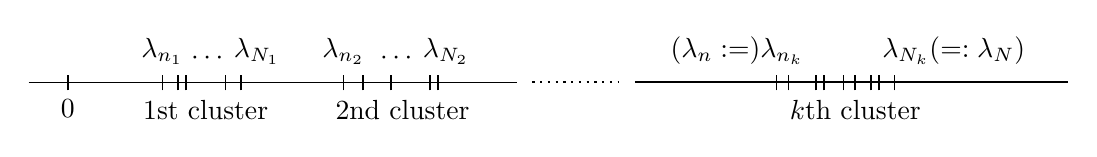
\begin{tikzpicture}[scale=1]
\newcommand{\tlen}{0.1}
\newcommand{\tick}[1]{\draw [semithick] (#1,-\tlen)--(#1,\tlen);}
\draw [semithick] (0,0)--(6.2,0);
\draw [thick,dotted] (6.2+0.2,0)--(6.2+1.3,0);
\draw [thick] (6.2+1.5,0)--(6.2+7,0);

\tick{0.5}\node [below] at (0.5,-\tlen) {$0$};

\tick{1.7}\node [above] at (1.7,\tlen) {$\lambda_{n_1}$};
\tick{1.9}
\tick{2.5}\node [above] at (2.3,\tlen) {$\cdots$};
\tick{2}
\tick{2.7}
\node [above] at (2.9,\tlen) {$\lambda_{N_1}$};
\node [below] at (2.25,-\tlen) {$1$st cluster};

\tick{4}\node [above] at (4,\tlen) {$\lambda_{n_2}$};
\tick{4.25}
\tick{4.6}\node [above] at (4.7,\tlen) {$\cdots$};
\tick{5.1}
\tick{5.2}
\node [above] at (5.3,\tlen) {$\lambda_{N_2}$};
\node [below] at (4.75,-\tlen) {$2$nd cluster};

\tick{9.5}\node [above] at (9,\tlen) {$(\lambda_n:=)\lambda_{n_k}$};
\tick{9.65}
\tick{10}
\tick{10.1}
\tick{10.35}
\tick{10.5}
\tick{10.7}
\tick{10.8}
\tick{11}\node [above] at (11.75,\tlen) {$\lambda_{N_k}(=:\lambda_{N})$};
\node [below] at (10.5,-\tlen) {$k$th cluster};
%
% \draw [semithick] (9,0)--(9,4)--(5,4)--(5,2.5)--(4,2.5)--(4,4)--(0,4)--(0,0);
% %\draw [<-{>[scale=2]}, thin] (0,0.5)--(3,0.5);
% \draw [big arrowhead, thin] (0,3.25)--(4,3.25);
% \draw [big arrowhead, thin] (4,3.25)--(0,3.25);
% \node [below] at (2,3.25) {$\pi$};
% \draw [big arrowhead, thin] (4,3.25)--(5,3.25);
% \draw [big arrowhead, thin] (5,3.25)--(4,3.25);
% \node [above] at (4.5,3.25) {$\displaystyle\frac{\pi}{4}$};
% %\draw [big arrowhead, thin] (4,2.5)--(7,2.5);
% %\draw [big arrowhead, thin] (7,2.5)--(4,2.5);
% %\node [below] at (5.5,2.5) {$\pi$};
% \draw [big arrowhead, thin] (0.75,0)--(0.75,4);
% \draw [big arrowhead, thin] (0.75,4)--(0.75,0);
% \node [right] at (0.75,2) {$\pi$};
% %\draw [big arrowhead, thin] (3.5,1)--(3.5,2);
% %\draw [big arrowhead, thin] (3.5,2)--(3.5,1);
% %\node [right] at (3.5,1.5) {$\displaystyle\frac{\pi}{3}$};
\end{tikzpicture}
\caption{Clusters of eigenvalues on the real axis.}
\label{fi:clusters}
\end{figure}



Denoting by $\|\cdot\|$ the $L^2(\Omega)$ norm, the directed distances of spaces measured in the energy and $L^2$ norms are defined as follows.
\begin{equation}
\label{eq:Delta}
\delta_a(E_k, E_{h,k}) = \max_{\substack{v \in E_k\\ \|\nabla v \|=1}} \min_{ v_h \in E_{h,k}} \|\nabla v - \nabla v_h \|
,\quad
\delta_b(E_k, E_{h,k}) = \max_{\substack{v \in E_k\\ \| v \|=1}} \min_{ v_h \in E_{h,k}} \| v- v_h \|.
\end{equation}
% \cred{[Please, check carefully the notation in the above line. I replaced the old notation with hats by the new notation with $_h$.]}

%To measure the angle between two, in general non-orthogonal, spaces $E_{h,k}$ and $E_{h,K}$, 
% let us introduce 

For reader's convenience and for the later reference, we recall the recent error bounds from \cite{LiuVej2022}. 
Take $\rho$ such that 
$\lambda_n < \rho \leq \lambda_{N+1}$, then
{
\begin{align}
  \label{eq:Deltaest}
  \delta_a^2(E_k,E_{h,k})
  &\leq  {\frac{\rho (\hat\lambda^{(k)}_N -  \lambda_n)  + \lambda_n \hat\lambda^{(k)}_N \vartheta^{(k)}}{\hat\lambda^{(k)}_N(\rho - \lambda_n)}}
%  (=:\Delta^{(1)}(E_K,E_{h,K}) ), 
   \quad\text{and}
\\
  \label{eq:deltaest}
  \delta_b^2(E_k,E_{h,k})
  &\leq {\frac{\hat\lambda^{(k)}_N - \lambda_n + \theta^{(k)}}{\rho - \lambda_n}},
\end{align}
where
\begin{align*}
  \hat\lambda^{(k)}_N &= \max_{v_h \in E_{h,k}} \frac{\norm{\nabla v_h}^2}{\norm{v_h}^2},
\quad
  \vartheta^{(k)} = \sum_{\ell=1}^{k-1} \left( \frac{\rho}{ \lambda_{n_\ell} } - 1 \right) \left[ \hat{\zeta}(E_{h,\ell},E_{h,k}) + \delta_a(E_\ell,E_{h,\ell}) \right]^2, 
  %\quad\text{and}
\\
  \theta^{(k)} &= \sum_{\ell=1}^{k-1} \left(\rho - \lambda_{n_\ell}\right) \left[ \hat{\varepsilon}(E_{h,\ell},E_{h,k}) + \delta_b(E_\ell,E_{h,\ell}) \right]^2.
\end{align*}
Note that quantities
\begin{equation*}
  %\label{eq:defeps}
  \hat{\zeta}(E_{h,\ell},E_{h,k}) = \max_{\substack{v\in E_{h,\ell}\\ \|\nabla v\|=1}} \max_{\substack{w\in E_{h,k}\\ \|\nabla w\|=1}} (\nabla v, \nabla w),
\quad
  \hat{\varepsilon}(E_{h,\ell},E_{h,k}) = \max_{\substack{v\in E_{h,\ell}\\ \| v\|=1}} \max_{\substack{w\in E_{h,k}\\ \|w\|=1}} ( v , w )
\end{equation*}
}%
%
% \begin{align}
%   \label{eq:Deltaest}
%   \delta_a^2(E_K,E_{h,K})
%   &\leq  {\frac{\rho (\hat\lambda^{(K)}_N -  \lambda_n)  + \lambda_n \hat\lambda^{(K)}_N \vartheta^{(K)}}{\hat\lambda^{(K)}_N(\rho - \lambda_n)}}
% %  (=:\Delta^{(1)}(E_K,E_{h,K}) ), 
%   \quad\text{and}
% \\
%   \label{eq:deltaest}
%   \delta_b^2(E_K,E_{h,K})
%   &\leq {\frac{\hat\lambda^{(K)}_N - \lambda_n + \theta^{(K)}}{\rho - \lambda_n}},
% \end{align}
% where
% \begin{align*}
%   \hat\lambda^{(K)}_N &= \max_{\hat v \in E_{h,K}} \frac{\norm{\nabla \hat v}^2}{\norm{\hat v}^2},
% \quad
%   \vartheta^{(K)} = \sum_{k=1}^{K-1} \left( \frac{\rho}{ \lambda_{n_k} } - 1 \right) \left[ \hat{\zeta}(E_{h,k},E_{h,K}) + \delta_a(E_k,E_{h,k}) \right]^2, 
%   %\quad\text{and}
% \\
%   \theta^{(K)} &= \sum_{k=1}^{K-1} \left(\rho - \lambda_{n_k}\right) \left[ \hat{\varepsilon}(E_{h,k},E_{h,K}) + \delta_b(E_k,E_{h,k}) \right]^2.
% \end{align*}
% Note that quantities
% \begin{equation*}
%   %\label{eq:defeps}
%   \hat{\zeta}(E_{h,k},E_{h,K}) = \max_{\substack{v\in E_{h,k}\\ \|\nabla v\|=1}} \max_{\substack{w\in E_{h,K}\\ \|\nabla w\|=1}} (\nabla v, \nabla w),
% \quad
%   \hat{\varepsilon}(E_{h,k},E_{h,K}) = \max_{\substack{v\in E_{h,k}\\ \| v\|=1}} \max_{\substack{w\in E_{h,K}\\ \|w\|=1}} ( v , w )
% \end{equation*}
measure the non-orthogonality between spaces of approximate eigenfunctions for the previous clusters and can be easily computed by using \cite[Lemma~2]{LiuVej2022}.
{Further}
{note that in \cite{LiuVej2022}, the approximate eigenfunction $\{u_{h,i}\}$ 
are considered as %can be provided in an 
arbitrary and the orthogonality of $\{u_{h,i}\}$ is not required.}





\section{Projection error-based estimate in the $L^2$ norm}
\label{se:optimalL2}

% In the standard theory of the finite element method applied to boundary value problems, the error estimates in the $L^2$ norm can be derived by using the Aubin--Nitsche technique.
The result of \cite[Theorem 8.1]{Boffi:2010}, and the explicitly known value of the constant in the \emph{a priori} error estimate for the energy projection \cite{LiuOis2013} enable us to mimic this approach for the eigenvalue problem and derive an optimal order convergent guaranteed and fully computable upper bound on the directed distance of the exact and approximate spaces of eigenfunctions measured in the $L^2(\Omega)$-norm.

%\begin{remark}\label{rem:hat_u_i_and_u_i_h}
First, we mention that $u_{h,i}$ is not available in practical computation, in general, because it is a result of a
generalized matrix eigenvalue solver polluted typically by rounding errors and truncation errors of iterative algorithms. 
In principle, 
{we could apply the interval arithmetic to have a rigorous representation of $u_{h,i}$,}
{but such} argument would make the paper lengthy and not easy to read. Therefore, we concentrate here on a theoretical analysis of the discretization error $(u_{h,i}-u_i)$,
{where $u_{h,i}$ is the exact solution of the discrete problem \eqref{eq:eig_pro_with_fem}.}
%\end{remark}

For the reader's convenience, we recall several results about the \emph{a priori} error estimates for finite element solutions of the Poisson equation. These \emph{a priori} error estimates will play an important role in subsequent error bounds for eigenfunctions.

%\paragraph{The Poisson equation} 
Given $f\in L^2(\Omega)$, let $u\in H_0^1(\Omega)$ be the weak solution of the Poisson problem satisfying
$$
(\nabla u, \nabla v) = (f,v) \quad \forall v \in H^1_0(\Omega).
$$
The corresponding Galerkin approximation $u_h \in V_h(\subset H^1_0(\Omega))$ is determined by the identity
$$
(\nabla u_h, \nabla v_h) = (f,v_h) \quad \forall v_h \in V_h.
$$
The energy projector $P_h : H_0^1(\Omega) \rightarrow V_h$ is defined by 
$(\nabla (u - P_h u), \nabla v_h) = 0$ for all $v_h \in V_h$. Clearly,  $u_h = P_h u$.

In \cite{LiuOis2013}, Liu proposed the following constructive \emph{a priori} error estimate with a computable constant $C_h$:
\begin{equation}
\label{eq:Ch}
\|\nabla(u-P_h u) \| \le C_h \|f\|, \quad \| u - P_h u \| \le C_h \| \nabla(u-P_h u) \| \le C_h^2 \|f\|
\end{equation}
and the following lower eigenvalue bounds:
\begin{equation}
\lambda_{k} \ge \frac{\lambda_{h,k}}{1+C_h^2 \lambda_{h,k}}~\quad (k=1, 2,\cdots, \operatorname{dim}(V_h)).    
\end{equation}
%-----------------------------------------------------------
\iffalse
\cred{Do we need the first inequality? It is included in the second one. If you think it can be deleted, please, remove it. If not, keep it.}
\cblue{It depends. For some non-conforming FEM space $V_h$, we can evaluate $C_h$ in $ \| u - P_h u \| \le C_h \| \nabla(u-P_h u) \|$ directly and without additional cost, compared with the hypercircle method which has to solve a side problem.}
\cred{So, would you like to keep it as it is? (It is fine with me.)}
\cblue{Yes.leave it unchanged. There is no pace to discuss the non-conforming case. }
\fi
%-----------------------------------------------------------
%
%\begin{remark}
In case of non-convex domains, the value of $C_h$ can be computed by solving a dual saddle-point problem based on the hypercircle method; see \cite[Sections 3.2--3.3]{LiuOis2013}. 
In case of convex domains, the value of $C_h$ can be easily computed by considering the Lagrange interpolation error constant; see \cite[Theorem~3.1]{LiuOis2013}. 
% \cred{[Xuefeng, please, is this statement correct in arbitrary dimension? If not, we should write here ``In case of two dimensional convex domains ...''.]}
% \cblue{Yes, "$C_h$ can be easily computed by considering the Lagrange interpolation error constant" holds for even for 3D case. I am wondering that is it necessary to provide reference for 3D case; for example, the work of Kobayashi--Tsuchiya on 3D interpolation constants.}
% \cred{[Good point. Please add the reference to the work of Kobayashi and Tsuchiya right after ``see \cite[Theorem~3.1]{LiuOis2013}''.]}
The specific value of $C_h$ is provided below in Section~\ref{se:numex} for the considered examples.
%\end{remark}


Throughout this section, we consider an arbitrary cluster of eigenvalues $\lambda_n, \lambda_{n+1}, \dots, \lambda_N$.
We denote by 
$\mathcal{C} = \{n, n + 1, \dots, N\}$
%$\mathcal{C}(k) = \{n_k, n_k + 1, \dots, N_k\}$ 
the set of indices of eigenvalues in this cluster
and by $|\mathcal{C}| = N - n + 1$ their number.
Spaces of exact and finite element eigenfunctions corresponding to this clusters are 
$E = \linspan\{ u_i : i \in \mathcal{C} \}$ and
$E_h = \linspan\{ u_{h,i} : i \in \mathcal{C} \}$, respectively.

It is also assumed that 
\begin{equation}    \label{eq:no_overlap_of_eigs}
\lambda_{h,n-1} < \lambda_n, \quad \lambda_N < \lambda_{h,N+1}.
\end{equation}
Such an assumption makes it possible to define the following quantities:
% \cred{[I think that the right conditions to assume are $\lambda_{h,n-1} < \lambda_n$ and $\lambda_N < \lambda_{h,N+1}$.]}
\begin{equation*}
\tau = \max_{j \in \mathcal{C}}\max_{i {\in}\mathcal{I} \setminus \mathcal{C}}\frac{\lambda_j}{|\lambda_{h,i}-\lambda_j|}
,\quad
\tau_h = \max_{j \in \mathcal{C}}\max_{i {\in}\mathcal{I} \setminus \mathcal{C}}\frac{\lambda_{h,i}}{|\lambda_{h,i}-\lambda_j|},
\end{equation*}
where $\mathcal{I} = \{1,2,\dots,\operatorname{dim} (V_h)\}$ stands for the set of all indices.
These quantities extend the one in \cite[pages 53, 57]{Boffi:2010} and have their origin in \cite{raviart1983introduction}. 
The application of the quantity $\tau $ can be found in \cite[Prop.~3.1]{CarGed2011}. The result in  Lemma~\ref{thm:u_and_pi_k_u} can be regarded an improvement of the one of \cite{CarGed2011}.

To derive 
% optimal order convergent guaranteed
the projection error-based 
% and fully computable 
upper bound 
on the directed distance of the exact and approximate spaces of eigenfunctions measured in the $L^2(\Omega)$-norm
by applying estimates \eqref{eq:Ch}, we need to
bound the error of the $L^2(\Omega)$ orthogonal projection $\Pi^\mathcal{C}_h: H^1_0(\Omega) \rightarrow E_h$ 
by the error of the energy projection $P_h: H^1_0(\Omega) \rightarrow V_h$. To achieve this goal, we first introduce several quantities and two auxiliary lemmas. 

%The number of indices in $\mathcal{C}$ is denoted by $|\mathcal{C}| = N - n + 1$.
%$E_{h,k} = \linspan\{u_{h,n_k}, u_{h,{n_k+1}},\dots,u_{h,N_k}\}$. 
%The $L^2(\Omega)$ orthogonal projector from $L^2(\Omega)$ to $E_{h,k}$ is denoted by $\Pi_{h,k}$.\cred{[$\Pi^\mathcal{C}_h$]}




\medskip


% The following lemma will be helpful in evaluating $\tau_k$ and $\tau_{h,k}$.
% \begin{lemma} 
% \label{lem:g_monotonicity}
% Given $\lambda_{h,i} (i\notin \mathcal{C}_k)$, define $$
% g(t):=\frac{t}{|\lambda_{h,i}-t|},\quad
% g_h(t):=\frac{\lambda_{h,i}}{|\lambda_{h,i}-t|}~.
% $$
% Then, it holds that, for $t \in [\lambda_n, \lambda_N]$,
% $$
% g(t) \le \max(g(\lambda_n), g(\lambda_N)), ~ %g(\lambda_N), ~
% g_h(t) \le \max(g_h(\lambda_n), g_h(\lambda_N))~.
% $$  
% \end{lemma}
% \begin{proof}
% From the assumption of \eqref{eq:no_overlap_of_eigs}, either 
% $t<\lambda_{h,i}$ or  $t>\lambda_{h,i}$ holds. 
% It is easy to see that both $g(t)$ and $g_h(t)$ are monotonic functions for either case.
% Thus,  the extreme values of $g$ and $g_h(t)$ are obtained at ends of the interval $[\lambda_n,\lambda_N]$.       
% \end{proof}

% For $k$th cluster of eigenfunction, introduce  $\beta_k$ 
Let us introduce the unit ball $E^B := \{ u \in E : \|u\|=1 \}$.
For the given cluster of eigenfunction, we introduce $\beta$ 
as the optimal (minimal) quantity  that makes the 
inequality 
\begin{equation}
 \label{def:beta}
 % \max_{\substack{}}
 \|(I-\Pi^\mathcal{C}_h) P_h u\| \le 
\beta 
  \max_{\substack{v \in E^B}} \|v - P_h v\| \quad 
  \mbox{hold for any } u\in E^B
 ~,
\end{equation}
% as the following quantity
% \begin{equation}
%     \label{def:beta}
% % \beta_k = \frac{\displaystyle \max_{\substack{u\in E_k, \|u\|=1}} \|(I-{\Pi}_{h,k}) P_h u\|}{\displaystyle 
% %   \max_{\substack{u \in E_k, \|u\|=1}} \|u - P_h u\|}.
% \beta := \frac{\displaystyle \max_{u\in E^B} \|(I-\Pi^\mathcal{C}_h) P_h u\|}{\displaystyle 
%   \max_{u \in E^B} \|u - P_h u\|},
% \end{equation}
and aim to obtain an upper bound of $\beta$.
In case $\|u - P_h u\|=0$ for all $u\in E^B$, it is natural to define $\beta=0$. 
Given $u =\sum_{j\in \mathcal{C}} c_j u_j \in E^B$,
let $\kappa:E^B \to E^B$ be the mapping such that
\begin{equation}
	\label{eq:def-kappa-h}
\kappa u = 
%\frac{1}{\overline{\lambda}}
\overline{\lambda}^{-1}
\sum_{j\in \mathcal{C}} {c_j \lambda_j}  u_j,\quad 
\text{where}\quad
{\overline{\lambda}^2} =\sum_{j\in \mathcal{C}}c_j^2 \lambda_j^2 .
\end{equation}
%
It is easy to see that $\kappa:E^B \to E^B$ is bijective.
We set $\overline u = \kappa u$, define the relative width $\xi := (\lambda_N - \lambda_n)/\lambda_n$ of the eigenvalue cluster of interest, and note that the following estimate holds:
%for $\|u-\overline{u}\|$:
$$
%\|u-\overline{u}\| = \sqrt{\sum_{j\in \mathcal{C}(k) } c_j^2 (1-\lambda_j/\overline{\lambda})^2 } \le \xi_k 
%:= \frac{\lambda_N-\lambda_n}{\lambda_n} 
\|u-\overline{u}\|^2 = \sum_{j\in \mathcal{C} } c_j^2 (1-\lambda_j/\overline{\lambda})^2 \le \xi^2. 
$$
%Here, $\xi_k$ is the relative width of the $k$th eigenvalue cluster.


\begin{lemma}\label{thm:u_and_pi_k_u}
%\LIU{[Maybe it is not necessary to mention the partition of clusters here, which is already done in \S 2.]}
Given an arbitrary clusters of eigenvalues, 
the quantity $\beta$ satisfies
% the following estimate holds:
% \begin{equation}
% \label{eq:thm_u_and_pi_k_u}
% \max_{\substack{u\in E_k \\ \|u\|=1}} \|u-{\Pi}_{h,k} u\| \le \eta_k \max_{\substack{u\in E_k \\ \|u\|=1}} \|u - P_h u\|
% \end{equation}
\begin{equation}
    \label{eq:est_of_beta_k}
    \beta \leq \tau  |\mathcal{C}|^{1/2}.
\end{equation}
% \begin{equation}
% \label{eq:thm_u_and_pi_k_u}
% \beta  \leq \left\{
% \begin{array}{ll}
% \tau_k     & \mbox{ if } \lambda_n=\lambda_N\\
% \tau_k  \sqrt{|\mathcal{C}(k)|}     & \mbox{otherwise}
% \end{array}\right. ~.
% \end{equation}
Further, if 
\begin{equation}
    \label{eq:condition_for_lemma}
\tau_h\xi < 1 - |\mathcal{C}|^{-1/2}
\end{equation}
then %a sharper estimation is available:
\begin{equation}
    \label{eq:est_of_beta_k_sharper}
    \beta \leq \frac{\tau}{1-\tau_h\xi} ~.
    % \cred{\sout{~(\le \tau |\mathcal{C}|^{1/2})}}.
\end{equation}
% \cred{[In my opinion, the bound $...(\le \tau |\mathcal{C}|^{1/2})$ is not need at all I suggest to remove it. If you think it worth it, please, mention it as a remark below the proof.]}
% As a direct result, in case of $\lambda_n=\lambda_{N}$, we have $\beta_k \le \tau_k$.

% \cred{[The lemma should state just pure facts and no comments. Therefore, I suggest to move comments that the second bound is sharper and what happens for $\lambda_n = \lambda_N$ below the proof of the lemma. See below.]}
\end{lemma}
\begin{remark}
Note that if condition \eqref{eq:condition_for_lemma} is satisfied than the estimate \eqref{eq:est_of_beta_k_sharper} is always sharper then the bound \eqref{eq:est_of_beta_k}.
Further, a smaller relative width of the cluster $\xi$  leads to a sharper upper bound \eqref{eq:est_of_beta_k_sharper}.
 In the extreme case of a multiple eigenvalue such that $\lambda_n=\lambda_N$, we have $\xi = 0$ and hence $\beta \le \tau$.
\end{remark}

\begin{proof}
%First, let us consider the case that $\lambda_{n}=\lambda_{N}$. 
%In this case, $\xi_k=0$. 
{First, for 
 $u_j \in E^B$ as an eigenfunction, let us apply the standard argument (see, e.g., \cite{Boffi:2010}) to show that
 $\|(I - \Pi^\mathcal{C}_h) P_h u_j\| \le \tau \| (I - P_h) u_j\|$. }
 Note that
$$
(I - \Pi^\mathcal{C}_h) P_h u_j = \sum_{i \in \mathcal{I} \setminus \mathcal{C}} (P_h u_j, u_{h,i}) u_{h,i} \in V_h,
$$
which leads to 
\begin{equation}
\label{eq:IPik}
\|(I  - \Pi^\mathcal{C}_h ) P_h u_j\|^2 = \sum_{i \in \mathcal{I} \setminus \mathcal{C}} (P_h u_j, u_{h,i})^2\:.
\end{equation}
In equality
\begin{equation}
    \label{eq:equality_in_lemma}
\lambda_{h,i} (P_h u_j , u_{h,i}) = (\nabla P_h u_j, \nabla u_{h,i})
= (\nabla u_j, \nabla u_{h,i}) = \lambda_j (u_j,u_{h,i}),
\end{equation}
we subtract $\lambda_j (P_h u_j,u_{h,i})$ on both sides and obtain
$$
(P_h u_j, u_{h,i}) = \frac{\lambda_j}{\lambda_{h,i} -\lambda_j } (u_j - P_h u_j,u_{h,i}).
$$
Summation over $i \in \mathcal{I}\setminus\mathcal{C}$ gives
$$
\sum_{i \in \mathcal{I} \setminus \mathcal{C}} (P_h u_j, u_{h,i})^2 \le \tau^2 \sum_{i \in \mathcal{I} \setminus \mathcal{C}} (u_j - P_h u_j,u_{h,i})^2 \le \tau^2 \|u_j - P_h u_j\|^2,
$$
where the last inequality follows form the identity $\sum_{i \in \mathcal{I}} (u_j - P_h u_j,u_{h,i})^2 = \| \Pi_h(u_j - P_h u_j) \|^2$ with $\Pi_h : H^1_0(\Omega) \rightarrow V_h$ denoting the $L^2(\Omega)$ orthogonal projector.
Using this in \eqref{eq:IPik}, we finally derive 
\begin{equation}
\label{eq:est_for_single_uj}
\|(I - \Pi^\mathcal{C}_h) P_h u_j\| \le \tau \| (I - P_h) u_j\|.
\end{equation}
%\LIU{Hence, $\beta_k\le \tau_k$ when $\lambda_{n}=\lambda_{N}$.}

% In case $\lambda_n = \lambda_N$, this estimate immediately implies the statement \eqref{eq:thm_u_and_pi_k_u}.

Next, %for a general case that $\lambda_n\not=\lambda_N$ is allowed, 
we consider any $u \in E^B$ and express it in the form $u =\sum_{j\in \mathcal{C}} c_j u_j$ with $\sum_{j\in\mathcal{C}} c_j^2 = 1$. 
%
Denoting the linear operator $(I - \Pi^\mathcal{C}_h) P_h $ by $L$,
% $$
% L u = \sum_{j \in \mathcal{C}(k)}c_j L u_j
% $$
the estimate \eqref{eq:est_for_single_uj} leads to
$$
\|L u \|^2 = \left\| \sum_{j \in \mathcal{C}}  c_j L u_j \right\|^2 \le \sum_{j \in \mathcal{C}} \|Lu_j\|^2    \le \tau^2 \sum_{j \in \mathcal{C}}  \| (I - P_h) u_j\|^2.
$$
Thus, we can estimate $\|(I - \Pi^\mathcal{C}_h) P_h u\|$ as
\begin{equation}
\label{eq:lemma_estimate_for_general_u_ver0}
\|(I - \Pi^\mathcal{C}_h) P_h u \| \le  
 \tau  |\mathcal{C}|^{1/2} \max_{u \in E^B} \|u - P_h u\|
\end{equation}
and statement \eqref{eq:est_of_beta_k} easily follows.

Finally, we consider the case when the condition \eqref{eq:condition_for_lemma} holds true. 
Given $u\in E^B$, we take $\overline{u}=\kappa u$ and $\overline{\lambda}$ as defined in \eqref{eq:def-kappa-h}.
% The proof is based on the following triangle inequality.
% \begin{equation}
% \label{eq:lem_triangle_inequality_new_}
%  \|u - \Pi_{h,k} u \| \le \|u - \Pi_{h,k} P_h u \| \le
%  \|u - P_h u \| + 
% \|P_h u-\Pi_{h,k} P_h u  \| .
% \end{equation}
%
Using inequality \eqref{eq:equality_in_lemma}, we obtain for $u$ the identity
$$
\lambda_{h,i} (P_h u , u_{h,i}) 
% = 
% (\nabla P_h u, \nabla u_{h,i})
%  = (\nabla u, \nabla u_{h,i})
% = (\sum_{j\in \mathcal{C}(k)} c_j \nabla u_j, \nabla u_{h,i}) 
= \overline{\lambda} (\overline{u},u_{h,i}).
$$
Subtracting $\overline{\lambda} (P_h \overline{u},u_{h,i})$ on both sides, we derive
$$
\left( \lambda_{h,i} P_h (u - \overline{u}) 
+ (\lambda_{h,i}
 -\overline{\lambda}) P_h \overline{u} , u_{h,i} \right) = \overline{\lambda} (\overline{u} -P_h \overline{u} ,u_{h,i}).
$$
Thus, 
$$
(P_h \overline{u}, u_{h,i}) = \frac{\overline{\lambda}}{\lambda_{h,i} -\overline{\lambda} } ( \overline{u} - P_h \overline{u},u_{h,i})
- 
\frac{\lambda_{h,i}}{\lambda_{h,i} -\overline{\lambda} } 
(P_h (u - \overline{u}), u_{h,i}).
$$
Since function $g(t)=t/ |\lambda_{h,i}-t|$ satisfies
$g(t) \le \max(g(\lambda_n), g(\lambda_N))$ for all $t \in [\lambda_n, \lambda_N]$
and function $g_h(t)=\lambda_{h,i}/|\lambda_{h,i}-t|$ is bounded in the same way, we have
%With the quantities $\tau_k$ and  $\tau_{h,k}$ and Lemma \ref{lem:g_monotonicity}, we have
$$
|(P_h \overline{u}, u_{h,i})| \leq \tau |\left(( I - P_h) \overline{u},u_{h,i}\right)| + \tau_h
|(P_h (u - \overline{u}), u_{h,i})|.
$$
Now, considering these inequalities for $i\in\mathcal{I}\setminus\mathcal{C}$, using the geometric inequality\footnote{
Given  vectors $a=(a_1, \cdots, a_n), b=(b_1, \cdots, b_n), c=(c_1, \cdots, c_n)$ with $a_i,b_i,c_i>0$ and
$a_i\leq b_i+c_i$, then their Euclidean norms satisfy
$\|a\| \le \|b\|+\|c\|.$
}
and the general fact that 
$\sum_{i\in \mathcal{I}\setminus\mathcal{C}} (\varphi,u_{h,i})^2
% \sout{= \| (\Pi_h - \Pi^\mathcal{C}_h)\varphi \|^2}
= \| (I - \Pi^\mathcal{C}_h) \Pi_h \varphi \|^2$ for any $\varphi \in H^1_0(\Omega)$ with $\Pi_h: H^1_0(\Omega) \rightarrow V_h$ being the $L^2(\Omega)$ orthogonal projector,  
% \LIU{[Now, it is O.K. Please confirm my inline suggestion.]}
%\le \| \varphi_h \|^2$
%for $\varphi_h := (I-P_h) \overline{u}$.
%Summation the above terms over $i\not\in \mathcal{C}(k)$ and application of the geometric inequalities 
we derive the bound
\begin{equation}
\label{eq:sub_inequality_1}    
\|(I-\Pi^\mathcal{C}_h)P_h {\overline{u}}\| \le 
\tau \|\overline{u}-P_h \overline{u}\| + 
\tau_h
\|(I-\Pi^\mathcal{C}_h)P_h (u - \overline{u})\|.
\end{equation}
%
%\begin{eqnarray*}
%&& \sqrt{\sum_{i \in \mathcal{C} \setminus \mathcal{C}(k)} (P_h \overline{u}, u_{h,i})^2 }\\
% &\le & 
%\sum_{i \in \mathcal{C} \setminus \mathcal{C}(k)} 
%(1+\beta) \tau_k^2  (\overline{u} - P_h \overline{u},u_{h,i})^2 
%+ (1+1/\beta) \tau_{h,k}^2 
%(P_h (u - \overline{u}), u_{h,i}) ^2
%\\
%%&\le & 
%%(1+\beta) \tau_k^2 \sum_{i \in \mathcal{C} \setminus \mathcal{C}(k)} (\overline{u} - P_h \overline{u},u_{h,i})^2 
%%+ (1+1/\beta) \tau_{h,k}^2 
%%\|(I-\Pi_{h,k})P_h (u-\overline{u})\|^2 
%%\\
%&\le & (1+\beta)  \tau_k^2 \|\overline{u} - P_h \overline{u}\|^2~ + (1+1/\beta)\tau_{h,k} ^2
%\|(I-\Pi_{h,k}) P_h (u-\overline{u})\|^2 .	
%\end{eqnarray*}
Since $\|u-\overline{u}\| \le \xi $, the definition of $\beta$ gives
% \cred{[I do not see this, but I see that $\|(I-\Pi_{h,k}) P_h (u-\overline{u})\|
% \le \xi_k$.]}
% \LIU{[Sorry for my mistake. The following inequality is about $\beta_k$ but not $\eta_k$.]}
% \cred{[OK, I see. But how $\xi_k$ appears here? (I am sorry, I am tired, so I am probably overlooking something. I will check it carefully later. However, tomorrow I will likely have no time.)]}
% \LIU{[ 
% Yesterday, I wrote down the proof with mistake as I was tired. Well, maybe we should slow down.  The paper is not in an urgent status. The deadline can be possibly extended. HINT: $u-\overline{u} \in E_k$ and its norm is less than $\xi_k$, which causes the appearance of $\xi_k$ in the following estimation.]}
% \cred{[I see, now. It is correct. Sorry for my slowness.]}
\begin{equation}
    \label{eq:sub_inequality_2}
\|(I-\Pi^\mathcal{C}_h) P_h (u-\overline{u})\|
\le 
\xi \beta \max_{u \in E^B} \|u - P_h u\|.
\end{equation}
Inequalities \eqref{eq:sub_inequality_1} and  \eqref{eq:sub_inequality_2} lead to the relation
% \cred{[OK]}
\begin{equation}
\label{eq:lemma_estimate_for_general_u_2}
\|(I - \Pi^\mathcal{C}_h) P_h \overline{u} \| \le  
\left( \tau   + \tau_h \xi  \beta \right)
 \max_{u \in E^B} \|u - P_h u\|.
\end{equation}
%
Since $\overline u = \kappa u$ and $\kappa: E^B \to E^B$ is a bijection, we have
$$
  \max_{u\in E^B} \|(I - \Pi^\mathcal{C}_h) P_h \kappa u \| 
= \max_{u\in E^B} \|(I - \Pi^\mathcal{C}_h) P_h u \|.
$$
Consequently, 
from the bound \eqref{eq:lemma_estimate_for_general_u_2} and the definition of $\beta$, we obtain
$$
\beta \le  \tau   + \tau_h \xi \beta.
$$
% \cred{[I see this step, if $\|(I - \Pi_{h,k}) P_h \overline{u} \| \leq \|(I - \Pi_{h,k}) \overline{u} \|$, but is it true?]}
% 
Since condition \eqref{eq:condition_for_lemma} implies $1-\tau_h\xi>0$, the estimate \eqref{eq:est_of_beta_k_sharper} follows.
\end{proof}

In next lemma, we show the relation between $\delta_b(E,E_h)$ and the projection error using the quantity $\beta$. 

\begin{lemma}\label{thm:u_and_pi_k_u_new_ver}
For the given cluster of eigenvalues, 
the following estimate holds:
\begin{equation}
\label{eq:thm_u_and_pi_k_u_new_}
\delta_b(E,E_h) = \max_{u\in E^B} \|u-\Pi^\mathcal{C}_h u\| \le 
(1+\beta)
  \max_{u \in E^B} \|u - P_h u\|.
 \end{equation}
% \cred{[The parenthesis around $\delta_b$ did not look good. I suggest to remove them.]} 
\end{lemma}
%

%
\begin{proof}
For any $u\in E^B$, since $\Pi^\mathcal{C}_h u$ provides the best approximation of $u$ under the $L^2$ norm in $E_h$, we have
\begin{equation}
\label{eq:lem_triangle_inequality_new_}
\|u - \Pi^\mathcal{C}_h u \| 
 \le \|u - \Pi^\mathcal{C}_h P_h u \| 
 \le \|u - P_h u \| + \|P_h u-\Pi^\mathcal{C}_h P_h u  \| .
\end{equation}
% \cred{[Why the red inequality holds true?]}\LIU{[See the  appended argument.]}
% \cred{[Excellent, many thanks.]}
Using the definition of the quantity $\beta$, we easily draw the conclusion.
\end{proof}
\begin{remark}
\label{remark:comparison_carsten_gedick}
In Proposition 3.2 of \cite{CarGed2011}, with $m:=|\mathcal{C}|=N-n+1$, the following result is obtained: For $u_{h,j} $ in $E$ as an eigenfunction associated to $\lambda_{h,j}$, 
$$
\min_{u\in E} \|u_{h,j}-u\| \le 
\sqrt{2} m(2m+1)(1+\tau)
 \max_{u_j\in E^B} \|u_j-P_h u_j\|~.
$$
If such a result is applied to  $\delta_b(E,E_h)$, one can obtain the following estimate.
\begin{equation}
\label{eq:overestimation}    
\delta_b(E,E_h) \le \sqrt{2} m(2m+1)(1+\tau)   \max_{u \in E^B} \|u - P_h u\|~.
\end{equation}
This bound is larger than the result in Lemma~\ref{thm:u_and_pi_k_u_new_ver}.
%Compared with the result in Lemma \ref{thm:u_and_pi_k_u_new_ver}, the above result provides an overestimation. 
Particularly, if
the eigenvalue cluster is tight, i.e., $\xi\approx 0$, we have $\beta\approx \tau$ and the bound %estimate 
\eqref{eq:overestimation} %has the overestimation
is overestimated by the factor $\sqrt{2} m(2m+1)$.
\end{remark}

Bounding $\beta$ by Lemma~\ref{thm:u_and_pi_k_u}, the following theorem presents
%Now, we formulate and prove 
the main result.

% \LIU{[I suggest to remove the theorem below, since it can not tell the convergence rate directly if the behavior of $\Delta (E_k, {E}_{h,k})$ is unknown.]}
% \cred{[I agree.]}


% \begin{theorem}\label{th:main}
% %For $k$th cluster, we have
% The following estimate
% \begin{equation}
% \label{eq:l2_norm_optimal_old_}
% \delta(E_k,E_{h,k})  \le \sqrt{\lambda_{N_k}} C_h \overline{\eta} \Delta (E_k, {E}_{h,k})
% %\cred{(=:\delta^{(2)}(E_K,E_{h,K}) )}
% \end{equation}
% holds for all $k=1,2,\dots,K$. 
% \end{theorem}
% \begin{proof}
% Consider the energy orthogonal projector $P_{h,k} : H^1_0(\Omega) \rightarrow E_{h,k}$.
% %with respect to the energy inner product $(\nabla \cdot, \nabla \cdot)$.
% By the definition of the distance $\Delta(E_k,E_{h,k})$ 
% % \begin{equation*}
% % %\label{eq:delta2}
% %   \Delta(E_k,E_{h,k}) = \max_{\substack{v \in E_k \\ \norm{\nabla v} = 1}} \norm{v - P_{h,k} v},
% % \end{equation*}
% we have for any $u\in E_k$, $\|\nabla u\|=1$ inequality
% $$
% \|\nabla(u-P_{h,k} u) \| \le \max_{\substack{v \in E_k \\ \norm{\nabla v} = 1}} \norm{\nabla v - \nabla P_{h,k} v} = \Delta (E_k, {E}_{h,k}).
% $$
% The {\em a priori} error estimate \eqref{eq:Ch} and the fact that $P_h u$ is the closest element to $u$ in $V_h$ yield
% \begin{equation}
%     \label{eq:local_est_1}
%     \|u-P_h u\| \le C_h \|\nabla(u-P_h u)\| \le C_h \|\nabla(u-P_{h,k} u)\| \le C_h \Delta (E_k, {E}_{h,k}).
% \end{equation}

% Definition of $\delta(E_k,E_{h,k})$ and bound \eqref{eq:thm_u_and_pi_k_u} give
% \begin{equation}
%     \label{eq:est2}
% \delta(E_k,E_{h,k}) = \max_{\substack{u\in E_k\\ \|u\|=1}} \|u-\Pi_{h,k} u\|
%   \leq  \overline{\eta}  \max_{\substack{u \in E_k\\ \|u\|=1 }} \| u - P_h u \|.
% \end{equation}
% Since inequality 
% ${\|\nabla u\| }/{\|u\|} \le \sqrt{\lambda_{N_k}}$ holds for all $u \in E_k$, we easily obtain bound
% \begin{equation}
%     \label{eq:est3}
%   \max_{\substack{u \in E_k\\ \|u\|=1 }} \| u - P_h u \| 
% = \max_{\substack{u \in E_k\\ \|\nabla u\|=1 }} \frac{1}{\|u\|} \| u - P_h u \| 
% \leq \sqrt{\lambda_{N_k}} \max_{\substack{u \in E_k\\ \|\nabla u\|=1 }} \| u - P_h u \|. 
% \end{equation}
% Combination of \eqref{eq:est2}, \eqref{eq:est3}, and \eqref{eq:local_est_1} finishes the proof.
% \end{proof}


\begin{theorem}\label{th:main_new_}
%For $k$th cluster, we have
Let $\beta$ be the quantity defined in \eqref{def:beta}.
For an arbitrary cluster of eigenvalues, 
the following estimate holds:
%
\begin{equation}
\label{eq:l2_norm_optimal}
\delta_b(E,E_h)  \le (1+\beta) {\lambda_N} C_h^2~.
%\cred{(=:\delta^{(2)}(E_K,E_{h,K}) )}
\end{equation}
% \cred{\sout{
% Here, $\beta$ is the quantity defined in \eqref{def:beta} and its explicit estimation is given in Lemma \ref{thm:u_and_pi_k_u}.}
% [The fact about the definition of $\beta$ should be mentioned in the assumptions of the Theorem and the remark about Lemma 1 should be outside of the Theorem.]
% }
\end{theorem}

\begin{proof}
Given $u\in E_k$, $u = \sum_{j\in \mathcal{C}}c_j u_j$, let $\overline{u}=\kappa u$ and $\overline{\lambda}^2 = \sum_{j\in \mathcal{C}}c_j^2 \lambda_j^2$.
%
Then the identity 
$$
(\nabla u, \nabla v)= (\overline{\lambda}\overline{u}, v), \quad \forall v\in V,
$$
holds and the {\em a priori} error estimate \eqref{eq:Ch} with $f=\overline{\lambda}\overline{u}$ yields
\begin{equation}
    \label{eq:local_est_1_new}
    \|u-P_h u\| \le C_h^2 \| \overline{\lambda}\overline{u}\| \le C_h^2\lambda_N .
\end{equation}
%
Definition of $\delta_b(E,E_h)$ and bounds \eqref{eq:thm_u_and_pi_k_u_new_} and \eqref{eq:local_est_1_new} give
\begin{equation*}
    \label{eq:est2_new}
\delta_b(E,E_h) = \max_{u\in E^B} \|u-\Pi^\mathcal{C}_h u\|
  \leq (1+\beta) \max_{u \in E^B} \| u - P_h u \| \le (1+\beta) C_h^2 \lambda_N.
\end{equation*}
\end{proof}

\begin{remark}
\label{remark:convergence-rate}
The result \cite{LiuOis2013} shows how to compute the quantity $C_h$. For convex domains, the solution of the Poisson problem has the regularity $u\in H^2(\Omega)$ and, consequently, we have
$C_h=O(h)$ via the Lagrange interpolation error estimation. 
For non-convex domains, the solution $u$ belongs to 
$H^{1+\alpha}(\Omega)$, where $\alpha \in (0,1]$ depends on the angles of re-entrant non-convex corners. 
In this case, the value of $C_h$ is evaluated by the hypercircle method using the Raviart--Thomas FEM, and it is expected that 
$C_h=O(h^{\alpha})$.

 As {it} is pointed out in \cite[Theorem 9.13]{Boffi:2010}, the FEM solutions approximate the eigenfunction independently. 
 That is, even for non-convex domains, if an 
 eigenfunction has the $H^2$-regularity, then the FEM approximation to such an eigenfunction has the $O(h^2)$ convergence rate under $L^2$ norm.
Since the projection error in the estimation \eqref{eq:thm_u_and_pi_k_u_new_} is restricted to the function in $E$ for the specified eigenvalue cluster, the estimation of Lemma \ref{thm:u_and_pi_k_u_new_ver} is consistent with the theoretical analysis of \cite{Boffi:2010}.

The proposed estimation \eqref{eq:l2_norm_optimal} using $C_h$ has a defect that, in case of non-convex domains, for an eigenfunction with a better regularity, the proposed bound still keeps the degenerated convergence rate, which is because the {\em a priori} error estimation is considering the worst case for the projection error.  
 If the regularity for eigenfunction in $E$ is known, then the estimation in Theorem \ref{th:main_new_} can also be improved since the estimation only depends on the projection error for eigenfunctions in the specified cluster.
For example, in the case of an L-shaped domain of \S \ref{sec:l-shape},  
 the eigenfunction $u=\sin(\pi x)\sin (\pi y)$ associated to  $\lambda_3=2\pi^2$ has the 
$H^2$-regularity, thus one can take $C_h<0.493h$ (where $h$ is the largest leg length for right triangles in the triangulation) for FEM approximation using triangulation with right triangles. 
\end{remark}

%We wish to emphasize that bound \eqref{eq:l2_norm_optimal} has an optimal rate of convergence. Indeed, if eigenfunctions are sufficiently smooth then the energy error converges on a sequence of globally refined meshes as $\Delta (E_k, {E}_{h,k}) \approx h^p$. Similarly, the interpolation constant converges as $C_h \approx h^p$.
%[XUEFENG: IS THERE A PROOF? CAN WE REFER HERE TO SOME EXISTING RESULT?]
%Consequently the $L^2$ error bound \eqref{eq:l2_norm_optimal} achieves the optimal rate of convergence $h^{2p}$.
%

% ------------------

% TO DO:

% - We can easily show the following inequality between our distanced and the distance in \cite{CanDusMadStaVoh2020} 
% $$
% \hat\lambda_n \Delta(E,\hE) \leq \| \nabla (P - \hP) \|_{\sigma_2(\mathcal{H})},
% $$
% $$
% \delta(E,\hE) \leq \| P - \hP \|_{\sigma_2(\mathcal{H})}.
% $$
% Therefore, we can use the bounds from \cite{CanDusMadStaVoh2020} to bound $\Delta(E,\hE)$ and use \eqref{eq:l2_norm_optimal} to obtain improved bounds on $\delta(E,\hE)$.

% DO WE WANT TO POINT THIS OUT?
% \cred{[At this point, it seems to me that this remark does not fit to this paper. Do you agree?]}
% \LIU{[To keep the result concise, I suggest not to include detailed discussion of other approaches in this paper.]}
% ------------------

\begin{remark}
Theorem 3 in \cite{LiuVej2022} provides the following estimate:
\begin{equation}
  \label{eq:energy_by_L2}
  \delta_a^2(E,E_h) \leq {2 - 2 \lambda_n \left( \frac{1 - \delta_b^2(E,E_h) }{\lambda_N \lambda_{h,N}} \right)^{1/2}} ~,
\end{equation}
where the energy error $\delta_a(E,E_h)$ {is bounded by} the $L^2$ error $\delta_b(E,E_h)$. 
However, bound \eqref{eq:energy_by_L2} is not optimal for clusters of a positive widths, i.e., $\lambda_n<\lambda_{N}$. On the other hand, for clusters consisting of a simple or a multiple eigenvalue, we have $\lambda_n = \lambda_N$ and the bound \eqref{eq:energy_by_L2} has the optimal speed of convergence. Indeed, in this case, it can be easily shown that the right-hand side of \eqref{eq:energy_by_L2} is dominated by $|\lambda_{h,N} - \lambda_N|$ and the other terms, including $\delta_b^2(E,E_h)$ are of higher order.
{Consequently, bound \eqref{eq:energy_by_L2} combined with \eqref{eq:l2_norm_optimal} provides a guaranteed and fully computable error bound in the energy norm with the optimal speed of convergence for a cluster consisting of only one simple or multiple eigenvalue.}
\end{remark}

\iffalse
\begin{remark}\label{re:re2} 
Theorem 8.1 of \cite{Boffi:2010} proves the estimate
$$
\Delta(E_{h,K}, E_K) \le C(K) \sup_{v\in E_1\cup \cdots  \cup E_{K}, \|v\|=1} \|\nabla(v-P_h v)\|,
$$
where we use the notation of the current paper.
Although the explicit bound on $\Delta(E_{h,K}, E_K)$ is not given in \cite{Boffi:2010}, we believe that using the constant $C_h$ from \eqref{eq:Ch}, we can provide an explicit bound on $C(K)$ and $\|\nabla(v-P_h v)\|$ and, thus, 
an estimate for $\Delta(E_{h,K}, E_K)$. 
In our future work, we will derive this estimate and compare it with bounds derived in the current paper.
[DO WE WANT TO PROMISE THIS?] 
\cred{[What is your idea?]}
\LIU{[In Corollary 9.11 of \cite{Boffi:2010}, there is a stronger result. But be careful that the assumption there is that the cluster width is zero. In case of zero width of cluster, our result in \eqref{eq:energy_by_L2} already proves this property.]} \LIU{[As a conclusion, there is no direct evidence or idea that we can obtain the ``optimal" explicit estimation of $\delta_a$ for a cluster with different eigenvalues. So, the remark shall be further weakened or removed.]}
\cred{[OK, please, remove this remark completely. We do not need it for the current paper at all.]}
\end{remark} 

\fi



\section{Numerical examples}
\label{se:numex}

This section provides numerical examples to  illustrate the accuracy of proposed bounds on the directed 
distances of spaces of exact and approximate eigenfunctions. The first example is the Laplace eigenvalue problem \eqref{eq:modpro} in the unit square domain for which 
{the exact eigenvalues and eigenfunctions are well known.} 
The second example is the same problem considered 
{in a non-convex L-shaped domain where eigenfunctions may have singularities at the re-entrant corner.}

Both examples are computed in 
the floating point arithmetic and the influence of rounding errors is not taken into account
{for simplicity.} 
However, if needed, mathematically rigorous estimates could be obtained by employing the interval arithmetic \cite{moore2009introduction}.

% \begin{figure}[tbh]
%     \centering
%     \includegraphics[scale=0.5]{square_uniform.eps}
%     \caption{The uniform mesh in the unit square with mesh size $h=1/4$.}
%     \label{fi:square_domain_uniform_mesh}
% \end{figure}


% \begin{table}[tbh]
% \begin{center}
% \begin{tabular}{|c|l|}
% \hline
% Cluster & Eigenvalues   \\
% \hline
% 1 & $\lambda_1 = 2\pi^2$  \\
% \hline
% 2 & $\lambda_2 = \lambda_3 = 5\pi^2$   \\ 
% \hline
% 3 & $\lambda_4 = 8\pi^2$   \\ 
% \hline
% 4 & $\lambda_5 = \lambda_6 = 10\pi^2$  \\ 
% \hline
% \end{tabular}
% \caption{\label{ta:square_domain_clusters}The four leading clusters for the square.}
% \end{center}
% \end{table}


% \begin{figure}[tbhp]
%     \centering
%     %\includegraphics[width=0.48\textwidth]{sqrconv_Delta_A}\quad
%     %\includegraphics[width=0.48\textwidth]{sqrconv_Delta_B}
%     \includegraphics[width=\textwidth]{sqrconvBB_Delta}
%     \caption{%
%     [TO DO: CORRECT REFERENCES IN THE LEGEND]
%     Bounds on the error of spaces of eigenfunctions in the energy norm for the square domain and the first four clusters. The exact value of $\Delta(E_K,E_{h,K})$ for $K=1,2,3,4$ is plotted by the dotted line. 
%     %The original bound \eqref{eq:Deltaest} (solid lines), the iteratively improved bound (dashed line), and the exact directed distance (dotted lines) are presented for clusters consisting of single eigenvalues $\lambda_1$ and $\lambda_4$ (left panel) and for clusters $\{\lambda_2,\lambda_3\}$ and $\{\lambda_5,\lambda_6\}$ (right panel).
%     }
%     \label{fi:squareH1}
% \end{figure}

% \begin{figure}[tbhp]
%     \centering
%     %\includegraphics[width=0.48\textwidth]{sqrconv_dltL2_A}\quad
%     %\includegraphics[width=0.48\textwidth]{sqrconv_dltL2_B}
%     \includegraphics[width=\textwidth]{sqrconvBB_dltL2}
%     \caption{%
%     [TO DO: CORRECT REFERENCES IN THE LEGEND]
%     Bounds on the error of spaces of eigenfunctions in the $L^2$ norm for the square domain and the first four clusters. The exact value of $\delta(E_K,E_{h,K})$ for $K=1,2,3,4$ is plotted by the dotted line.
%     %The original bound \eqref{eq:deltaest} (solid lines), the iteratively improved bound (dashed line), and the exact directed distance (dotted lines) are presented for clusters consisting of single eigenvalues $\lambda_1$ and $\lambda_4$ (left panel) and for clusters $\{\lambda_2,\lambda_3\}$ and $\{\lambda_5,\lambda_6\}$ (right panel).
%     }
%     \label{fi:squareL2}
% \end{figure}

\subsection{The unit square domain}
\label{sec:unit_square}
Consider the Laplace eigenvalue problem with homogeneous Dirichlet boundary conditions in the unit square $\Omega=(0,1)^2$: 
find eigenvalues $\lambda_i \in \R$ and corresponding eigenfunctions $u_i \neq 0$ such that
\begin{equation}
\label{eq:modpro}
  -\Delta u_i = \lambda_i u_i \quad\text{in }\Omega;
  \qquad
  u_i = 0 \quad\text{on }\partial\Omega.
\end{equation}
%Remark~\ref{re:examples} shows how the weak formulation of this problem fits to the considered abstract context.
% \cred{\sout{The $a$- and $b$-norms correspond to the energy and $L^2(\Omega)$ norms, respectively.}
% [This is a general (not problem specific) fact that we should either mention at the beginning, at the place where we define $\delta_a$ and $\delta_b$ or not to comment it at all.]
%}


\begin{table}[ht]
\caption{\label{ta:square_domain_clusters}The four leading clusters for the unit square.}
\begin{center}
\begin{tabular}{|c|c|c|c|c|}
\hline
\rule[-2mm]{0cm}{6mm}{}
 Cluster & 1 & 2 & 3 & 4 \\
 \hline
\rule[-2mm]{0cm}{6mm}{}
Eigenvalues & $\lambda_1 = 2\pi^2$ &
 $\lambda_2 = \lambda_3 = 5\pi^2$  &
 $\lambda_4 = 8\pi^2$   & 
 $\lambda_5 = \lambda_6 = 10\pi^2$  \\ 
\hline
\end{tabular}
\end{center}
\end{table}


The exact eigenpairs are known analytically to be
$$
\lambda_{ij} = (i^2+j^2)\pi^2,\quad u_{ij}=\sin(i\pi x) \sin(j\pi y), \quad i,j=1,2,3, \dots.
$$
These eigenvalues are either simple or multiple
and we cluster them according to the multiplicity.
The first four clusters are listed in Table~\ref{ta:square_domain_clusters}.
Since the exact eigenvalues are known, we use them to evaluate error bounds. 
{To compute bounds \eqref{eq:Deltaest} and \eqref{eq:deltaest} for
the cluster $\{\lambda_{n}, \lambda_{n+1}, \cdots, \lambda_{N}\}$, 
we choose $\rho = \lambda_{N+1}$.
}

\begin{figure}[ht]
\begin{center}
    \includegraphics[scale=0.25]{square_uniform.eps}
\end{center}
\caption{\label{fig:uniform_mesh_square} The uniform mesh with $h=1/4$ for the unit square.%
}
\label{fi:squaremesh}
\end{figure}


{Problem \eqref{eq:modpro}} is discretized by the conforming finite element method using piecewise linear functions. The finite element mesh $\cT_h$ is chosen as the uniform triangulation consisting of
isosceles right triangles; 
{see Figure~\ref{fi:squaremesh} for an illustration.
% \sout{see the mesh with size $h=1/4$ in Figure~\ref{fi:squaremesh}.}
}
The projection error constant can be easily obtained through the interpolation error constant
{as}
$C_h\le h/0.493$.


{
For each cluster, we compute bounds on $\delta_b(E_k,E_{h,k})$ and $\delta_a(E_k,E_{h,k})$ by 
the estimate \eqref{eq:l2_norm_optimal} from Theorem~\ref{th:main_new_} and its combination with the relation \eqref{eq:energy_by_L2}, respectively.
We then compare these results with the bounds \eqref{eq:Deltaest} and \eqref{eq:deltaest} computed by Algorithm I of \cite{LiuVej2022}.
}
% \cred{\sout{
% applying the bound \eqref{eq:Deltaest}, 
%  \eqref{eq:deltaest} \cred{using} Algorithm I of \cite{LiuVej2022},
% and the newly proposed bounds \eqref{eq:l2_norm_optimal} 
% obtained in Theorem \ref{th:main_new_} along with the relation  \eqref{eq:energy_by_L2}. 
% }}

The convergence behavior of computed bounds for the four leading clusters is shown in Figure ~\ref{fig:unit-square-l2} and \ref{fig:unit-square-h1}.
The results confirm the expected optimal convergence rate $O(h^2)$ of the estimate \eqref{eq:l2_norm_optimal}
for {$\delta_b(E_k,E_{h,k})$}, and the sub-optimal rate $O(h)$ from Algorithm I of \cite{LiuVej2022}. 

The estimate by Algorithm II of \cite{LiuVej2022} can provide impressively sharp bounds and the optimal convergence rate for the error of approximate eigenfunctions under both $L^2$ and $H^1$ norms. Since such an approach needs more {effort to post-process the approximate eigenfunction, reconstruct the flux, and estimate the} residual error of the eigenfunction approximation, the comparison with Algorithm II of \cite{LiuVej2022} is omitted here.


\begin{figure}[htp]
    \centering
    \includegraphics[width=\textwidth]{Unitsquare_L2.eps}
    \caption{\label{fig:unit-square-l2}Bounds on the $L^2(\Omega)$ distances of spaces of eigenfunctions
    {$\delta_b(E_k,E_{h,k})$} for the square domain and four leading clusters of eigenvalues
    {$k=1,2,3,4$.}
    }
    
\end{figure}


\begin{figure}[htp]
    \centering
    \includegraphics[width=\textwidth]{Unitsquare_H1.eps}
    \caption{\label{fig:unit-square-h1}
    Bounds on the energy distances of spaces of eigenfunctions {$\delta_a(E_k,E_{h,k})$} for the square domain and the four leading clusters {$k=1,2,3,4$}.
    }
\end{figure}

\subsection{The L-shaped domain}
\label{sec:l-shape}
We consider the Laplace eigenvalue problem \eqref{eq:modpro} in the L-shaped domain $\Omega = (-1,1)^2\setminus(-1,0]^2$
to present the standard example with singularities of eigenfunctions
and also to demonstrate the versatility of the proposed method. We solve this problem by using the classical linear conforming finite element space over a uniform mesh.

\begin{figure}[ht]
    \centering
    \includegraphics[scale=0.4]{L_shape_mesh.eps}
    \caption{L-shaped domain and the initial mesh
    }
    \label{fig:l_shaped_domain}
\end{figure}

Since the exact eigenvalues are not known,
the eigenvalue bounds
are evaluated by using
two-sided bounds on eigenvalues, which were computed in \cite{liu2014high} 
and we list them in Table~\ref{tab:l_shaped_eig_lower_bound}. 
The first four eigenvalues are simple and form trivial clusters.
The values of the projection error constants are obtained by applying the hypercircle method proposed in \cite{LiuOis2013}; see Table \ref{table:lshape-projection-error-constant}.


\begin{table}[ht]
    \centering
    \caption{Lower bounds on the leading eigenvalues for the L-shaped domain.}
    \begin{tabular}{|c|c|c|c|c|}
    \hline
    \rule[-2mm]{0mm}{6mm}{}
    $\lambda_1$  & $\lambda_2$ &$\lambda_3$ & $\lambda_4$ & $\lambda_5$ \\
        \hline
    \rule[-2mm]{0mm}{6mm}{}
    $9.6397_{1}^{3}$ & $15.1972_{5}^{6}$ & $19.7392_0^1$ & $29.5214_7^9$ & $31.9126_2^4$ \\
        \hline
    \end{tabular}

    \label{tab:l_shaped_eig_lower_bound}
\end{table}


\begin{table}[h]
    \centering
    \caption{\label{table:lshape-projection-error-constant}Projection error constants}
    \begin{tabular}{|c|c|c|c|c|}
    \hline
    \rule[-2mm]{0mm}{6mm}{}
    $h$  & $1/32$ &$1/64$ & $1/128$ & $1/256$ \\
        \hline
    \rule[-2mm]{0mm}{6mm}{}
    $C_h$ & $0.0359$ & $0.0218$ & $0.0134$ & $0.00832$ \\
        \hline
    \end{tabular}

\end{table}

The initial finite element mesh is displayed in Figure~\ref{fig:l_shaped_domain}.
First, we apply the bounds \eqref{eq:Deltaest} and \eqref{eq:deltaest} to the four leading eigenvalue clusters. Since the exact error $\delta_b$ cannot be evaluated directly, we apply the residual error-based estimation, i.e., Algorithm II of \cite{LiuVej2022} to obtain a sharp bound of $\delta_b$. Numerical evaluation of such a bound implies that $\delta_b$ has the convergence rate as $O(h^{3/2})$ for the first cluster and $O(h^{2})$ for the rest $3$ clusters. 
Figure~\ref{fig:lshape-l2} shows the bounds on the $L^2(\Omega)$ distance $\delta_b$. 
Figure~\ref{fig:lshape-h1} compares the bounds on the energy distance $\delta_a$.
The results confirm that the newly proposed estimate of $\delta_b$ based on the projection error estimate, namely the estimate \eqref{eq:l2_norm_optimal} in Theorem~\ref{th:main_new_}, provides improved convergence rates in comparison with the bound \eqref{eq:deltaest}.
% \sout{The results confirm that the newly proposed estimation of $\delta_b$ provide an improved convergence rate than the bound \eqref{eq:deltaest} without using the projection error estimate.}

\begin{figure}[htp]
    \centering
    \includegraphics[width=\textwidth]{LShape_L2_with_REE.eps}
    \caption{\label{fig:lshape-l2}Bounds on the $L^2(\Omega)$ distances of spaces of eigenfunctions
    {$\delta_b(E_k,E_{h,k})$} for the L-shaped domain and four leading clusters {$k=1,2,3,4$}.
    }
\end{figure}


\begin{figure}[htp]
    \centering
    \includegraphics[width=\textwidth]{LShape_H1_N.eps}
    \caption{\label{fig:lshape-h1}Bounds on the energy distances of spaces of eigenfunctions {$\delta_a(E_k,E_{h,k})$} for the L-shaped domain and the four leading clusters {$k=1,2,3,4$}. 
    }
\end{figure}

% \subsection{The 2D dumbbell shaped domain}
% In this example, we again consider the Laplace eigenvalue problem \eqref{eq:modpro}, 
% but now in a dumbbell shaped domain consisting of two unit squares connected by a bar 
% of width $0.02$ and length $0.1$, see Figure~\ref{fi:dumbbell_domain}, 
% where also the initial mesh is depicted.

% The exact solution of this eigenvalue problem is not known, but the eigenvalues are expected 
% to be close to eigenvalues for a union of two squares, i.e., two eigenvalues close to 
% $2\pi^2 \approx 19.739$, four eigenvalues close to $5\pi^2 \approx 49.348$, etc.
% In order to compute high precision two-sided bounds for these eigenvalues, we
% combine the Crouzeix--Raviart nonconforming finite elements and 
% the Lehmann--Goerisch method as proposed in \cite{Liu2015}.
% The resulting two-sided bounds obtained on a fine mesh and finite element spaces of the third order
% are presented in Table~\ref{ta:dumbbell_domain_clusters}. 

% Table~\ref{ta:dumbbell_domain_clusters} also shows the chosen division of the first twelve eigenvalues into four clusters. 
% Note that eigenvalues $\lambda_3$ and $\lambda_4$ are strictly separated from $\lambda_5$ and $\lambda_6$. Therefore, they could be considered as two separate clusters, but then the spectral gap between them would be small and the factor $\rho - \lambda_n$ in \eqref{eq:Deltaest} and \eqref{eq:deltaest} would yield large overestimation. For this reason, all four eigenvalues $\lambda_3, \dots, \lambda_6$ are considered in one cluster.

% The value of $C_h$ in \eqref{eq:Ch} is computed for the mesh depicted in
% Figure~\ref{fi:dumbbell_domain} and for its five successive uniform refinements by using the method from \cite{LiuOis2013}. The obtained values are presented in Table~\ref{ta:value_of_ch}.

% \begin{table}[ht]
%     \centering
%     \begin{tabular}{|c|c|c|c|c|c|c|}
%     \hline
%      Refinement times   & 0 & 1 & 2 & 3 & 4 & 5 \\
%     \hline
%     $C_h$  & 0.0419 & 0.0233  & 0.0118 & 0.00588  & 0.00290  & 0.00155  \\
%     \hline
%     \end{tabular}
%     \caption{Values of $C_h$ for the dumbbell shaped domain and linear conforming finite elements. The first row indicates the number of uniform mesh refinements of the initial mesh shown in Figure~\ref{fi:dumbbell_domain}.}
%     \label{ta:value_of_ch}
% \end{table}

% We compute the bounds on $\Delta(E_K,E_{h,K})$ and $\delta(E_K,E_{h,K})$ for the four clusters $K=1,2,3,4$ as we did for the square domain. 
% Figure~\ref{fi:dumbbellH1} presents the bound \eqref{eq:Deltaest}, \eqref{eq:energy_by_L2}, and the iteratively improved bound for the energy norm. 
% The first and the third cluster are very tight and we observe the first order convergence. However, the convergence curves for the second and the fourth cluster bend due to the larger width of these clusters.
% Figure~\ref{fi:dumbbellL2} shows the bound \eqref{eq:deltaest}, \eqref{eq:l2_norm_optimal}, and its iterative improvement for the $L^2$ norm. 
% The second order convergence of bound \eqref{eq:l2_norm_optimal} and the first order convergence of \eqref{eq:deltaest} and of the iteratively improved bound are observed.

% \begin{figure}[htbp]
%     \centering
%     %\includegraphics[width=0.48\textwidth]{dmblconv_Delta_A}\quad
%     %\includegraphics[width=0.48\textwidth]{dmblconv_Delta_B}
%     \includegraphics[width=\textwidth]{dmblconvBB_Delta.eps}
%     \caption{%
%     [TO DO: CORRECT REFERENCES IN THE LEGEND]
%     Bounds on the error of spaces of eigenfunctions in the energy norm for the dumbbell shaped domain.
%     %The original bound \eqref{eq:Deltaest} (solid lines) and the iteratively improved bound (dashed line) are presented for the first two clusters in the left panel and for the next two clusters in the right panel.
%     }
%     \label{fi:dumbbellH1}
% \end{figure}

% \begin{figure}[htbp]
%     \centering
%     %\includegraphics[width=0.48\textwidth]{dmblconv_dltL2_A}\quad
%     %\includegraphics[width=0.48\textwidth]{dmblconv_dltL2_B}
%     \includegraphics[width=\textwidth]{dmblconvBB_dltL2.eps}
%     \caption{%
%     [TO DO: CORRECT REFERENCES IN THE LEGEND]
%     Bounds on the error of spaces of eigenfunctions in the $L^2$ norm for the dumbbell shaped domain. 
%     %The original bound \eqref{eq:deltaest} (solid lines) and the iteratively improved bound (dashed line) are presented for the first two clusters in the left panel and for the next two clusters in the right panel.
%     }
%     \label{fi:dumbbellL2}
% \end{figure}






\section{Conclusions}
\label{se:conclusions}

For finite element eigenfunctions, we derived 
a projection error-based
% an optimal order a posteriori error
bound on the $L^2$ 
distance $\delta_b$ by employing the explicitly 
known value of the constant {$C_h$} in the \emph{a priori} error estimate for the energy projection.
The obtained optimal estimate of $\delta_b$ can be further utilized to improve the bound for the energy distance $\delta_a$. 
The derived bound is fully computable and guaranteed. 


% \vskip 0.5cm
% 
% \paragraph{Acknowledgement.} The first author is supported by Japan Society for the Promotion of Science, Grand-in-Aid for Young Scientist (B) 26800090 and Grant-in-Aid for Scientific Research (C) 18K03411.
% The second author is supported by the Neuron Fund for Support of Science, project no.~24/2016, and by RVO 67985840.


%    Bibliographies can be prepared with BibTeX using amsplain,
%    amsalpha, or (for "historical" overviews) natbib style.
\bibliographystyle{amsplain}
%    Insert the bibliography data here.
\bibliography{vejchod_aee}

\end{document}

%%%%%%%%%%%%%%%%%%%%%%%%%%%%%%%%%%%%%%%%%%%%%%%%%%%%%%%%%%%%%%%%%%%%%%%%

%    Templates for common elements of a journal article; for additional
%    information, see the AMS-LaTeX instructions manual, instr-l.pdf,
%    included in the MCOM author package, and the amsthm user's guide,
%    linked from http://www.ams.org/tex/amslatex.html .

%    Section headings
\section{}
\subsection{}

%    Ordinary theorem and proof
\begin{theorem}[Optional addition to theorem head]
% text of theorem
\end{theorem}

\begin{proof}[Optional replacement proof heading]
% text of proof
\end{proof}

%    Figure insertion; default placement is top; if the figure occupies
%    more than 75% of a page, the [p] option should be specified.
\begin{figure}
\includegraphics{filename}
\caption{text of caption}
\label{}
\end{figure}

%    Mathematical displays; for additional information, see the amsmath
%    user's guide, linked from http://www.ams.org/tex/amslatex.html .

% Numbered equation
\begin{equation}
\end{equation}

% Unnumbered equation
\begin{equation*}
\end{equation*}

% Aligned equations
\begin{align}
  &  \\
  &
\end{align}

%-----------------------------------------------------------------------
% End of mcom-l-template.tex
%-----------------------------------------------------------------------
